\documentclass[10pt]{article}

\usepackage[utf8]{inputenc}
\usepackage[spanish]{babel}
\decimalpoint
\usepackage{amsmath, amssymb}
\usepackage{xcolor}
\usepackage{geometry}
\geometry{letterpaper, margin=1in}
\usepackage{graphicx}
\usepackage{float}
\usepackage{colortbl}
\usepackage{caption}
\usepackage{booktabs}
\usepackage{tabularx}
\usepackage{microtype}
\PassOptionsToPackage{hyphens}{url}
\usepackage{hyperref}
\hypersetup{
    colorlinks=true,
    breaklinks=true,
    linkcolor=blue,
    urlcolor=blue,
    citecolor=blue
}
\Urlmuskip=0mu plus 1mu\relax
\setlength{\emergencystretch}{3em}
%%%%%%%%%%%%%%%%%%%%%%%%%%%%%%%%%%%%%%%%%%%%%%%%%%%%%%%%%%%%%%%%%%%%%%%%%%%%%%%%%%%%%%%%%%%%%%%%%%%%%%%%%%%%%%%%%%%%%%%%%%%%%%%%%%%%%%%%%%%%%%%%%%%%%%%%%%%%%%%%%%%%%%%%%%%%%%%%%%%%%%%%%%%%%%
%%%%%%%%%%%%%%%%%%%%%%%%%%%%%%%%%%%%%%%%%%%%%%%%%%%%%%%%%%%%%%%%%%%%%%%%%%%%%%%%%%%%%%%%%%%%%%%%%%%%%%%%%%%%%%%%%%%%%%%%%%%%%%%%%%%%%%%%%%%%%%%%%%%%%%%%%%%%%%%%%%%%%%%%%%%%%%%%%%%%%%%%%%%%%%
\title{Universidad Panamericana \\ Maestría en Ciencia de Datos 
\\ Econometría \\ \vspace{0.5cm} 
Proyecto Final: Determinantes de Victorias en MLB
}

\author{Enrique Ulises Báez Gómez Tagle\\Luis Alejandro Guillén Alvarez\\Grupo2}
\date{\today}
%%%%%%%%%%%%%%%%%%%%%%%%%%%%%%%%%%%%%%%%%%%%%%%%%%%%%%%%%%%%%%%%%%%%%%%%%%%%%%%%%%%%%%%%%%%%%%%%%%%%%%%%%%%%%%%%%%%%%%%%%%%%%%%%%%%%%%%%%%%%%%%%%%%%%%%%%%%%%%%%%%%%%%%%%%%%%%%%%%%%%%%%%%%%%%
%%%%%%%%%%%%%%%%%%%%%%%%%%%%%%%%%%%%%%%%%%%%%%%%%%%%%%%%%%%%%%%%%%%%%%%%%%%%%%%%%%%%%%%%%%%%%%%%%%%%%%%%%%%%%%%%%%%%%%%%%%%%%%%%%%%%%%%%%%%%%%%%%%%%%%%%%%%%%%%%%%%%%%%%%%%%%%%%%%%%%%%%%%%%%%
\begin{document}

\maketitle

\tableofcontents

\newpage
%%%%%%%%%%%%%%%%%%%%%%%%%%%%%%%%%%%%%%%%%%%%%%%%%%%%%%%%%%%%%%%%%%%%%%%%%%%%%%%%%%%%%%%%%%%%%%%%%%%%%%%%%%%%%%%%%%%%%%%%%%%%%%%%%%%%%%%%%%%%%%%%%%%%%%%%%%%%%%%%%%%%%%%%%%%%%%%%%%%%%%%%%%%%%%
%%%%%%%%%%%%%%%%%%%%%%%%%%%%%%%%%%%%%%%%%%%%%%%%%%%%%%%%%%%%%%%%%%%%%%%%%%%%%%%%%%%%%%%%%%%%%%%%%%%%%%%%%%%%%%%%%%%%%%%%%%%%%%%%%%%%%%%%%%%%%%%%%%%%%%%%%%%%%%%%%%%%%%%%%%%%%%%%%%%%%%%%%%%%%%
\section{Introducción}
\subsection{Objetivo del trabajo:}
El propósito de este trabajo es aplicar un análisis de regresión lineal simple para identificar y cuantificar la relación entre las victorias de un equipo de béisbol en una temporada y distintos indicadores de desempeño ofensivo y defensivo. Este análisis permite entender en qué medida factores como la diferencia de carreras, la efectividad del pitcheo (ERA) o el número de jonrones influyen en los triunfos obtenidos. De esta forma, se busca mostrar cómo las técnicas econométricas pueden emplearse para explicar y pronosticar resultados deportivos.
%%%%%%%%%%%%%%%%%%%%%%%%%%%%%%%%%%%%%%%%%%%%%%%%%%%%%%%%%%%%%%%%%%%%%%%%%%%%%%%%%%%%%%%%%%%%%%%%%%%%%%%%%%%%%%%%%%%%%%%%%%%%%%%%%%%%%%%%%%%%%%%%%%%%%%%%%%%%%%%%%%%%%%%%%%%%%%%%%%%%%%%%%%%%%%
\subsection{Justificación:}
Las variables seleccionadas se eligieron por su relevancia directa en el rendimiento de un equipo de Grandes Ligas:
\begin{itemize}
    \item \textbf{Victorias (W):} representa el desempeño global de un equipo en una temporada, es el objetivo principal a explicar.
    \item \textbf{Diferencia de carreras (RunDiff = R - RA):} refleja la solidez ofensiva y defensiva combinada; se espera una relación positiva con las victorias.
    \item \textbf{ERA (Earned Run Average):} mide la calidad del pitcheo, donde un menor valor debería asociarse con más victorias (relación negativa).
    \item \textbf{Jonrones (HR):} indicador clave del poder ofensivo; se espera una relación positiva con las victorias.
    \item \textbf{Transformación logarítmica de HR (log(HR+1)):} se incluye como forma funcional alternativa para evaluar si la relación no es estrictamente lineal.
\end{itemize}
Con este análisis se espera comprobar qué variable tiene mayor poder explicativo sobre las victorias, así como evaluar la utilidad de las transformaciones funcionales para mejorar la capacidad predictiva.
%%%%%%%%%%%%%%%%%%%%%%%%%%%%%%%%%%%%%%%%%%%%%%%%%%%%%%%%%%%%%%%%%%%%%%%%%%%%%%%%%%%%%%%%%%%%%%%%%%%%%%%%%%%%%%%%%%%%%%%%%%%%%%%%%%%%%%%%%%%%%%%%%%%%%%%%%%%%%%%%%%%%%%%%%%%%%%%%%%%%%%%%%%%%%%
\subsection{Descripción de los datos:}
Se utiliza la Base de Datos de Béisbol de Lahman 1871-2024, publicada por la Society for American Baseball Research (SABR) con datos recopilados por Sean Lahman. La base está disponible en formato CSV, y específicamente se emplea el archivo \texttt{Teams.csv}, que contiene estadísticas anuales de desempeño de cada equipo de Grandes Ligas . 

El archivo original incluye 48 columnas y 3075 observaciones, correspondientes a temporadas desde 1871 hasta 2024. Sin embargo, para este trabajo se decidió filtrar únicamente los equipos de las ligas Americana (AL) y Nacional (NL), ya que representan las ligas principales de las Grandes Ligas de Béisbol y permiten obtener datos más homogéneos en términos de reglas y estructura competitiva. Asimismo, se seleccionó el periodo 2000-2019 porque corresponde a una etapa reciente del béisbol moderno, con un calendario estable de 162 juegos por temporada y sin las distorsiones que generó la temporada 2020 por la pandemia de COVID-19. Con este filtro se obtuvieron 600 observaciones (30 equipos por temporada durante 20 años), lo cual asegura un tamaño de muestra suficiente para aplicar análisis con validez estadística.

El dataset maestro conserva las siguientes variables principales:
\begin{itemize}
    \item Identificadores: \texttt{yearID}, \texttt{lgID}, \texttt{teamID}, \texttt{franchID}, \texttt{name}, \texttt{team\_year}, \texttt{season\_date}.
    \item Resultados: \texttt{W} (victorias), \texttt{L} (derrotas), \texttt{G} (juegos jugados).
    \item Estadísticas de desempeño: \texttt{R} (carreras anotadas), \texttt{RA} (carreras permitidas), \texttt{ERA} (efectividad), \texttt{HR} (jonrones).
    \item Variables derivadas: \texttt{RunDiff = R - RA}, \texttt{logHR1 = ln(HR+1)}.
\end{itemize}

El dataset es de tipo corte transversal en panel (equipo-año), con una observación por equipo por temporada, con esto es posible aplicar los modelos de regresión simple y realizar análisis descriptivos y de correlación.
%%%%%%%%%%%%%%%%%%%%%%%%%%%%%%%%%%%%%%%%%%%%%%%%%%%%%%%%%%%%%%%%%%%%%%%%%%%%%%%%%%%%%%%%%%%%%%%%%%%%%%%%%%%%%%%%%%%%%%%%%%%%%%%%%%%%%%%%%%%%%%%%%%%%%%%%%%%%%%%%%%%%%%%%%%%%%%%%%%%%%%%%%%%%%%
%%%%%%%%%%%%%%%%%%%%%%%%%%%%%%%%%%%%%%%%%%%%%%%%%%%%%%%%%%%%%%%%%%%%%%%%%%%%%%%%%%%%%%%%%%%%%%%%%%%%%%%%%%%%%%%%%%%%%%%%%%%%%%%%%%%%%%%%%%%%%%%%%%%%%%%%%%%%%%%%%%%%%%%%%%%%%%%%%%%%%%%%%%%%%%
\section{Selección de Variables}
\subsection{Variable dependiente:}
La variable dependiente seleccionada es el número de \textbf{victorias (W)} que obtiene cada equipo de las Grandes Ligas de Béisbol (MLB) en una temporada regular. Esta variable representa de manera directa el desempeño global de un equipo, ya que ganar más partidos es el objetivo principal dentro de una temporada. A partir de ella se busca explicar qué factores de rendimiento ofensivo y defensivo tienen mayor influencia en el éxito deportivo.
%%%%%%%%%%%%%%%%%%%%%%%%%%%%%%%%%%%%%%%%%%%%%%%%%%%%%%%%%%%%%%%%%%%%%%%%%%%%%%%%%%%%%%%%%%%%%%%%%%%%%%%%%%%%%%%%%%%%%%%%%%%%%%%%%%%%%%%%%%%%%%%%%%%%%%%%%%%%%%%%%%%%%%%%%%%%%%%%%%%%%%%%%%%%%%
\subsection{Variables independientes:}
Para el análisis de regresión simple se seleccionaron tres variables distintas, cada una analizada en un modelo separado:%%%%%%%%%%%%%%%%%%%%%%%%%%%%%%%%%%%%%%%%%%%%%%%%%%%%%%%%%%%%%%%%%%%%%%%%%%%%%%%%%%%%%%%%%%%%%%%%%%%%%%%%%%%%%%%%%%%%%%%%%%%%%%%%%%%%%%%%%%%%%%%%%%%%%%%%%%%%%%%%%%%%%%%%%%%%%%%%%%%%%%%%%%%%%%

\begin{itemize}
    \item \textbf{Diferencia de carreras (RunDiff = R - RA):} mide la diferencia entre las carreras anotadas (\texttt{R}) y las carreras permitidas (\texttt{RA}). Es un indicador directo del dominio de un equipo sobre sus rivales; se espera que un mayor diferencial de carreras se traduzca en un mayor número de victorias (\(\beta > 0\)). 
    \item \textbf{ERA (Earned Run Average):} representa el promedio de carreras limpias permitidas por cada nueve entradas lanzadas. Es una métrica clave de la calidad del pitcheo: un valor más bajo de ERA refleja un mejor desempeño de los lanzadores y, por lo tanto, debería estar negativamente correlacionado con las derrotas y positivamente con las victorias (\(\beta < 0\)). 
    \item \textbf{Jonrones (HR):} corresponde al número total de cuadrangulares conectados por un equipo en una temporada. Dado que los jonrones aportan carreras directas, se espera que tengan una relación positiva con las victorias (\(\beta > 0\)). Además, se incluirá una transformación funcional \(\log(HR+1)\) para evaluar si la relación entre jonrones y victorias presenta un comportamiento no lineal, suavizando el efecto de valores extremos.
\end{itemize}
%%%%%%%%%%%%%%%%%%%%%%%%%%%%%%%%%%%%%%%%%%%%%%%%%%%%%%%%%%%%%%%%%%%%%%%%%%%%%%%%%%%%%%%%%%%%%%%%%%%%%%%%%%%%%%%%%%%%%%%%%%%%%%%%%%%%%%%%%%%%%%%%%%%%%%%%%%%%%%%%%%%%%%%%%%%%%%%%%%%%%%%%%%%%%%
%%%%%%%%%%%%%%%%%%%%%%%%%%%%%%%%%%%%%%%%%%%%%%%%%%%%%%%%%%%%%%%%%%%%%%%%%%%%%%%%%%%%%%%%%%%%%%%%%%%%%%%%%%%%%%%%%%%%%%%%%%%%%%%%%%%%%%%%%%%%%%%%%%%%%%%%%%%%%%%%%%%%%%%%%%%%%%%%%%%%%%%%%%%%%%
\section{Análisis de Estadísticas Descriptivas}

\subsection{Medidas de tendencia central y dispersión:}
A partir del dateset maestro con las varibles y observaciones seleccionadas, se calculan las siguientes estadísticas descriptivas:
\begin{table}[H]
    \centering
    \begin{tabular}{lrrrrrrrrrrr}
        \hline
            Variable & Count & Mean & Median & Mode & Std & Var & Min & Q1 & Q3 & IQR & Max \\
        \hline
            W       & 600 & 80.97 & 81.00 & 86.00 & 11.79 & 138.92 & 43.00 & 72.00 & 90.00 & 18.00 & 116.00 \\
            RunDiff & 600 & 0.00  & 2.00  & 54.00 & 111.11 & 12344.79 & -337.00 & -87.00 & 81.25 & 168.25 & 300.00 \\
            ERA     & 600 & 4.25  & 4.21  & 4.01  & 0.53  & 0.29 & 2.94 & 3.86 & 4.60 & 0.74 & 5.71 \\
            HR      & 600 & 173.47 & 170.00 & 161.00 & 36.87 & 1359.12 & 91.00 & 148.00 & 199.00 & 51.00 & 307.00 \\
            logHR1  & 600 & 5.14  & 5.14  & 5.09  & 0.21  & 0.05 & 4.52 & 5.00 & 5.30 & 0.29 & 5.73 \\
            R       & 600 & 740.67 & 735.00 & 735.00 & 83.21 & 6924.21 & 513.00 & 684.00 & 795.25 & 111.25 & 978.00 \\
            RA      & 600 & 740.67 & 733.00 & 715.00 & 88.93 & 7909.25 & 525.00 & 676.75 & 804.00 & 127.25 & 981.00 \\
            G       & 600 & 161.96 & 162.00 & 162.00 & 0.31 & 0.10 & 161.00 & 162.00 & 162.00 & 0.00 & 163.00 \\
            L       & 600 & 80.97 & 80.50 & 76.00 & 11.76 & 138.34 & 46.00 & 72.00 & 90.00 & 18.00 & 119.00 \\
        \hline
    \end{tabular}
\end{table}

A continuación se detallan las características principales:

\begin{itemize}
    \item \textbf{Victorias (W):} En promedio los equipos ganan 81 juegos por temporada , con una desviación estándar de 11.8. El rango va de 43 a 116 victorias, lo que refleja tanto equipos altamente competitivos como equipos en el extremo opuesto.
    \item \textbf{Diferencia de carreras (RunDiff):} Tiene media cercana a cero, que sería esperado en un balance global de liga, pero una alta dispersión ($\approx 111$, rango de -337 a +300). Esto muestra que algunos equipos dominan ampliamente a sus rivales mientras otros son ampliamente superados.
    \item \textbf{ERA (Efectividad del pitcheo):} Promedia 4.25, con valores típicos entre 3.9 y 4.6 (IQR = 0.74). La dispersión es moderada y refleja diferencias en la calidad del pitcheo entre equipos, con casos extremos desde 2.94 hasta 5.71.
    \item \textbf{Jonrones (HR):} Los equipos conectan en promedio 173 cuadrangulares por temporada, con un rango entre 91 y 307. Esta variabilidad se ve reflejada por las distintas filosofías ofensivas.
    \item \textbf{Transformación logarítmica (logHR1):} Reduce la dispersión ($\approx 0.21$) y comprime la escala, aunque en este rango de valores la distribución sigue un patrón casi lineal respecto a HR.
    \item \textbf{Carreras anotadas (R) y recibidas (RA):} Ambas variables tienen media $\approx 741$, lo que es natural dado el equilibrio de la liga. Su dispersión ($\approx 83-89$) muestra diferencias en ofensiva y defensiva entre equipos.
    \item \textbf{Juegos (G):} Es prácticamente constante en 162, como dicta el calendario, con variaciones mínimas por suspensiones o ajustes.
    \item \textbf{Derrotas (L):} Presentan la misma estructura que las victorias, con media 81 y desviación de 11.7, dada la relación \(W+L \approx 162\).
\end{itemize}
%%%%%%%%%%%%%%%%%%%%%%%%%%%%%%%%%%%%%%%%%%%%%%%%%%%%%%%%%%%%%%%%%%%%%%%%%%%%%%%%%%%%%%%%%%%%%%%%%%%%%%%%%%%%%%%%%%%%%%%%%%%%%%%%%%%%%%%%%%%%%%%%%%%%%%%%%%%%%%%%%%%%%%%%%%%%%%%%%%%%%%%%%%%%%%
\subsection{Visualización de los datos:}

Con el fin de comprender mejor el comportamiento de las variables y su relación con las victorias, se generaron distintas visualizaciones: histogramas, boxplots, diagramas de dispersión, gráficas de pastel y una serie de tiempo de ejemplo.

\begin{figure}[H]
    \centering
    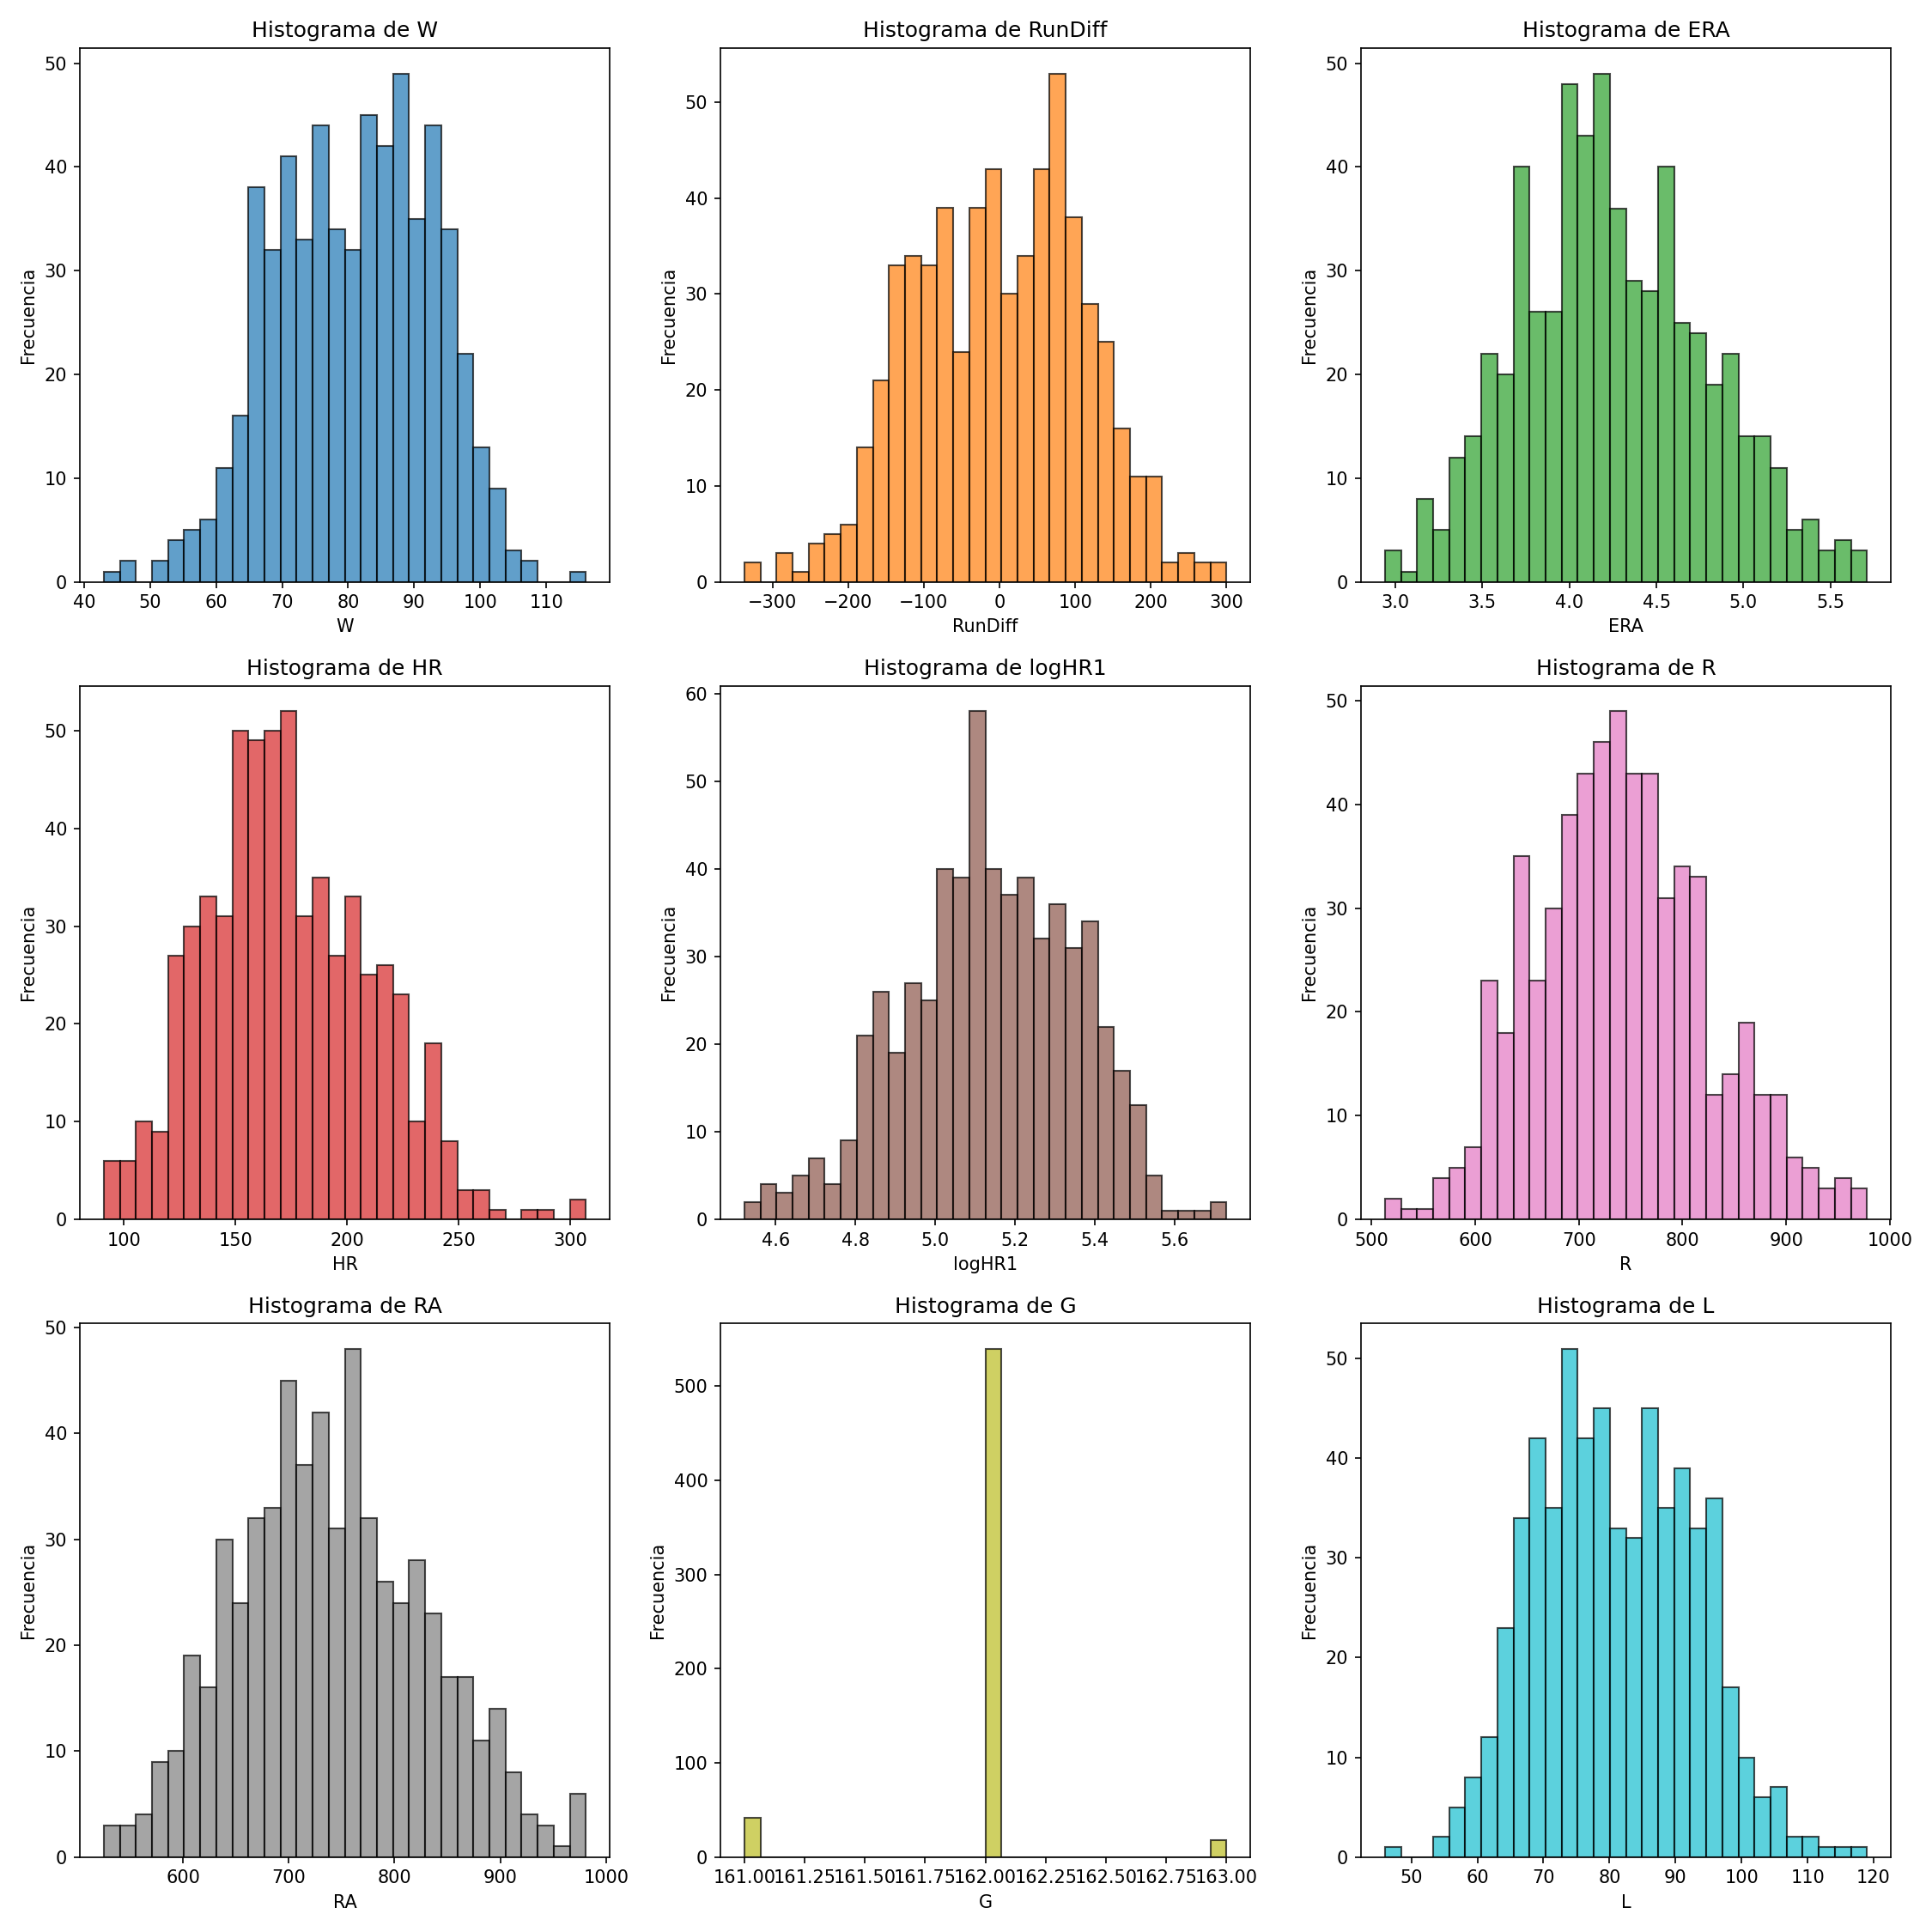
\includegraphics[width=0.65\textwidth]{../plots/all_histograms.png}
    \caption{Histogramas de W, RunDiff, ERA, HR, logHR1, R, RA, G y L (2000--2019).}
\end{figure}

Los histogramas confirman distribuciones aproximadamente simétricas en \textbf{W} y \textbf{L}, con centro en 81 victorias/derrotas. 
\textbf{RunDiff} muestra gran dispersión, confirmarndo que algunos equipos superan a sus rivales por cientos de carreras, mientras otros son ampliamente superados. 
\textbf{ERA} se concentra en torno a 4, reflejando diferencias moderadas en pitcheo. 
\textbf{HR} se distribuye entre 100-300, y su transformación \textbf{logHR1} comprime los valores extremos, suavizando colas. 
\textbf{R} y \textbf{RA} tienen formas parecidas, centradas cerca de 740, lo que refleja equilibrio ofensivo-defensivo en la liga. 
\textbf{G} es casi una constante en 162, validando la homogeneidad del calendario.\\

\begin{figure}[H]
    \centering
    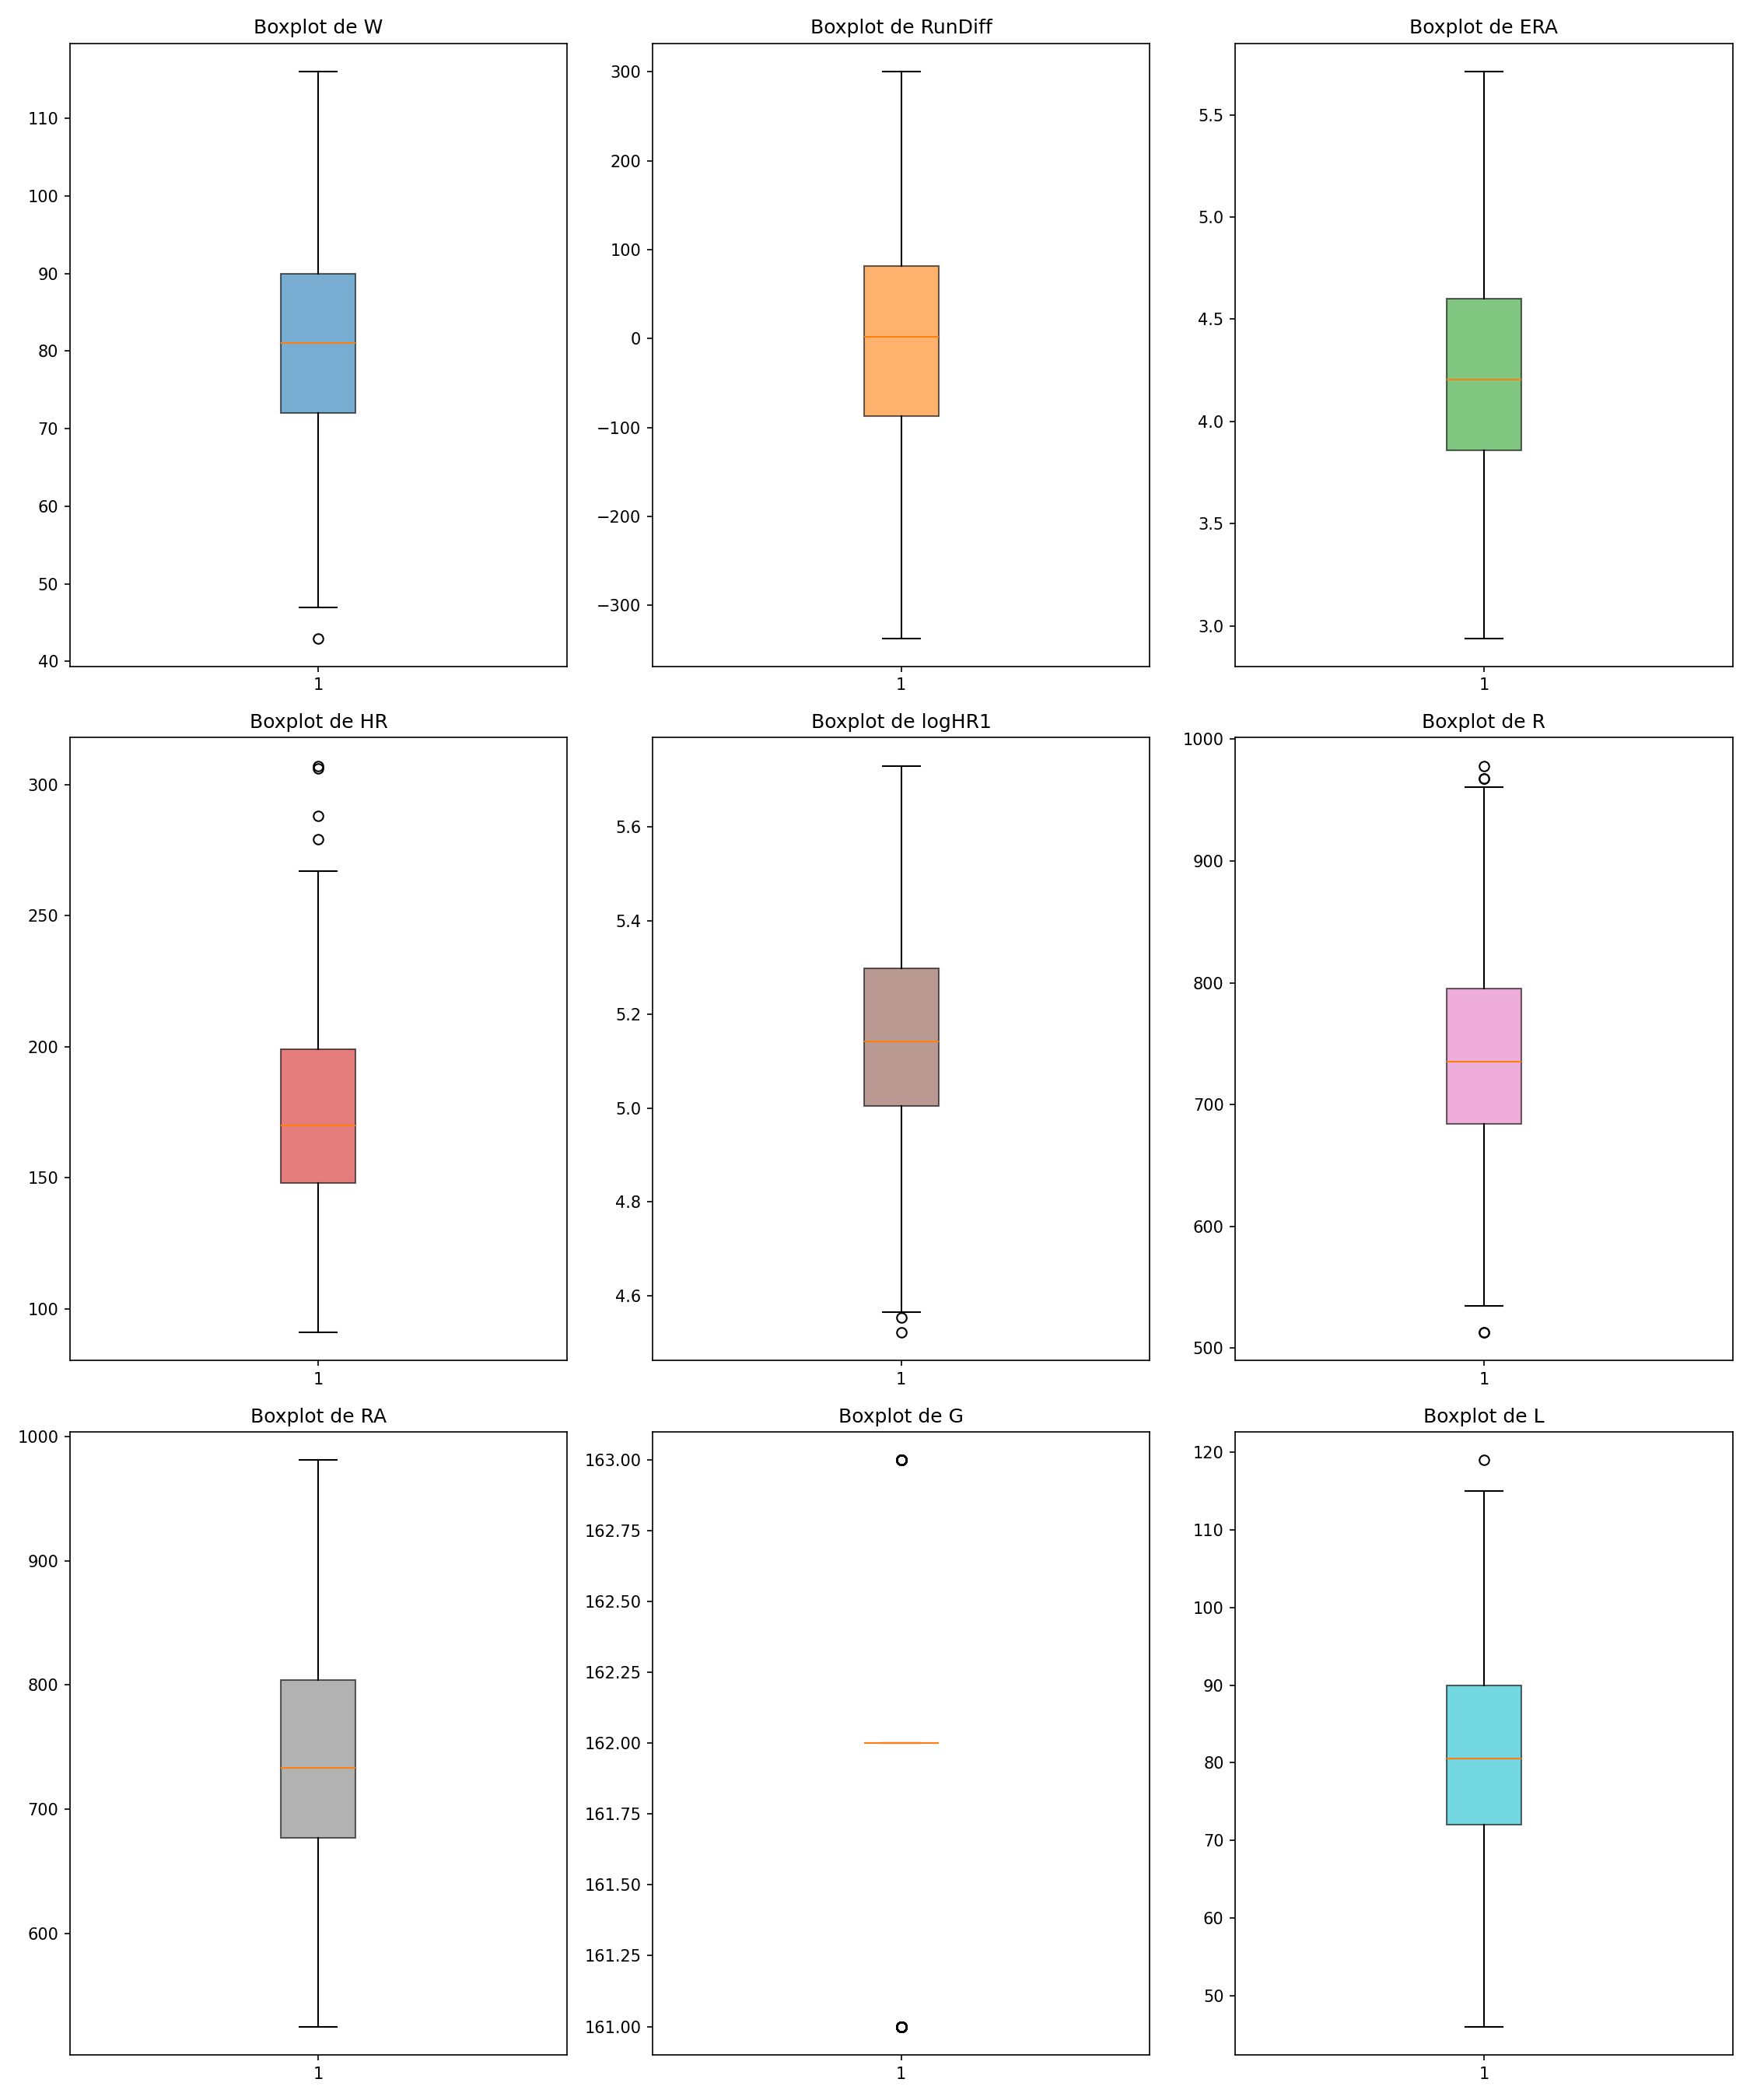
\includegraphics[width=0.7\textwidth]{../plots/all_boxplots.png}
    \caption{Boxplots por variable: dispersión, mediana y valores atípicos.}
\end{figure}

Los boxplots identifican \textit{outliers} relevantes: 
(i) en \textbf{HR}, equipos con poder ofensivo distintivo (300+ HR), 
(ii) en \textbf{R} se ven reflejados esos mismos casos extremos de producción ofensiva.
(iii) en \textbf{G}, ligeras desviaciones (161 o 163 partidos), explicadas por suspensiones o dobles juegos. 
En \textbf{RunDiff} se observan extremos tanto positivos como negativos, reflejando temporadas históricas dominantes o muy pobres.

\begin{figure}[H]
    \centering
    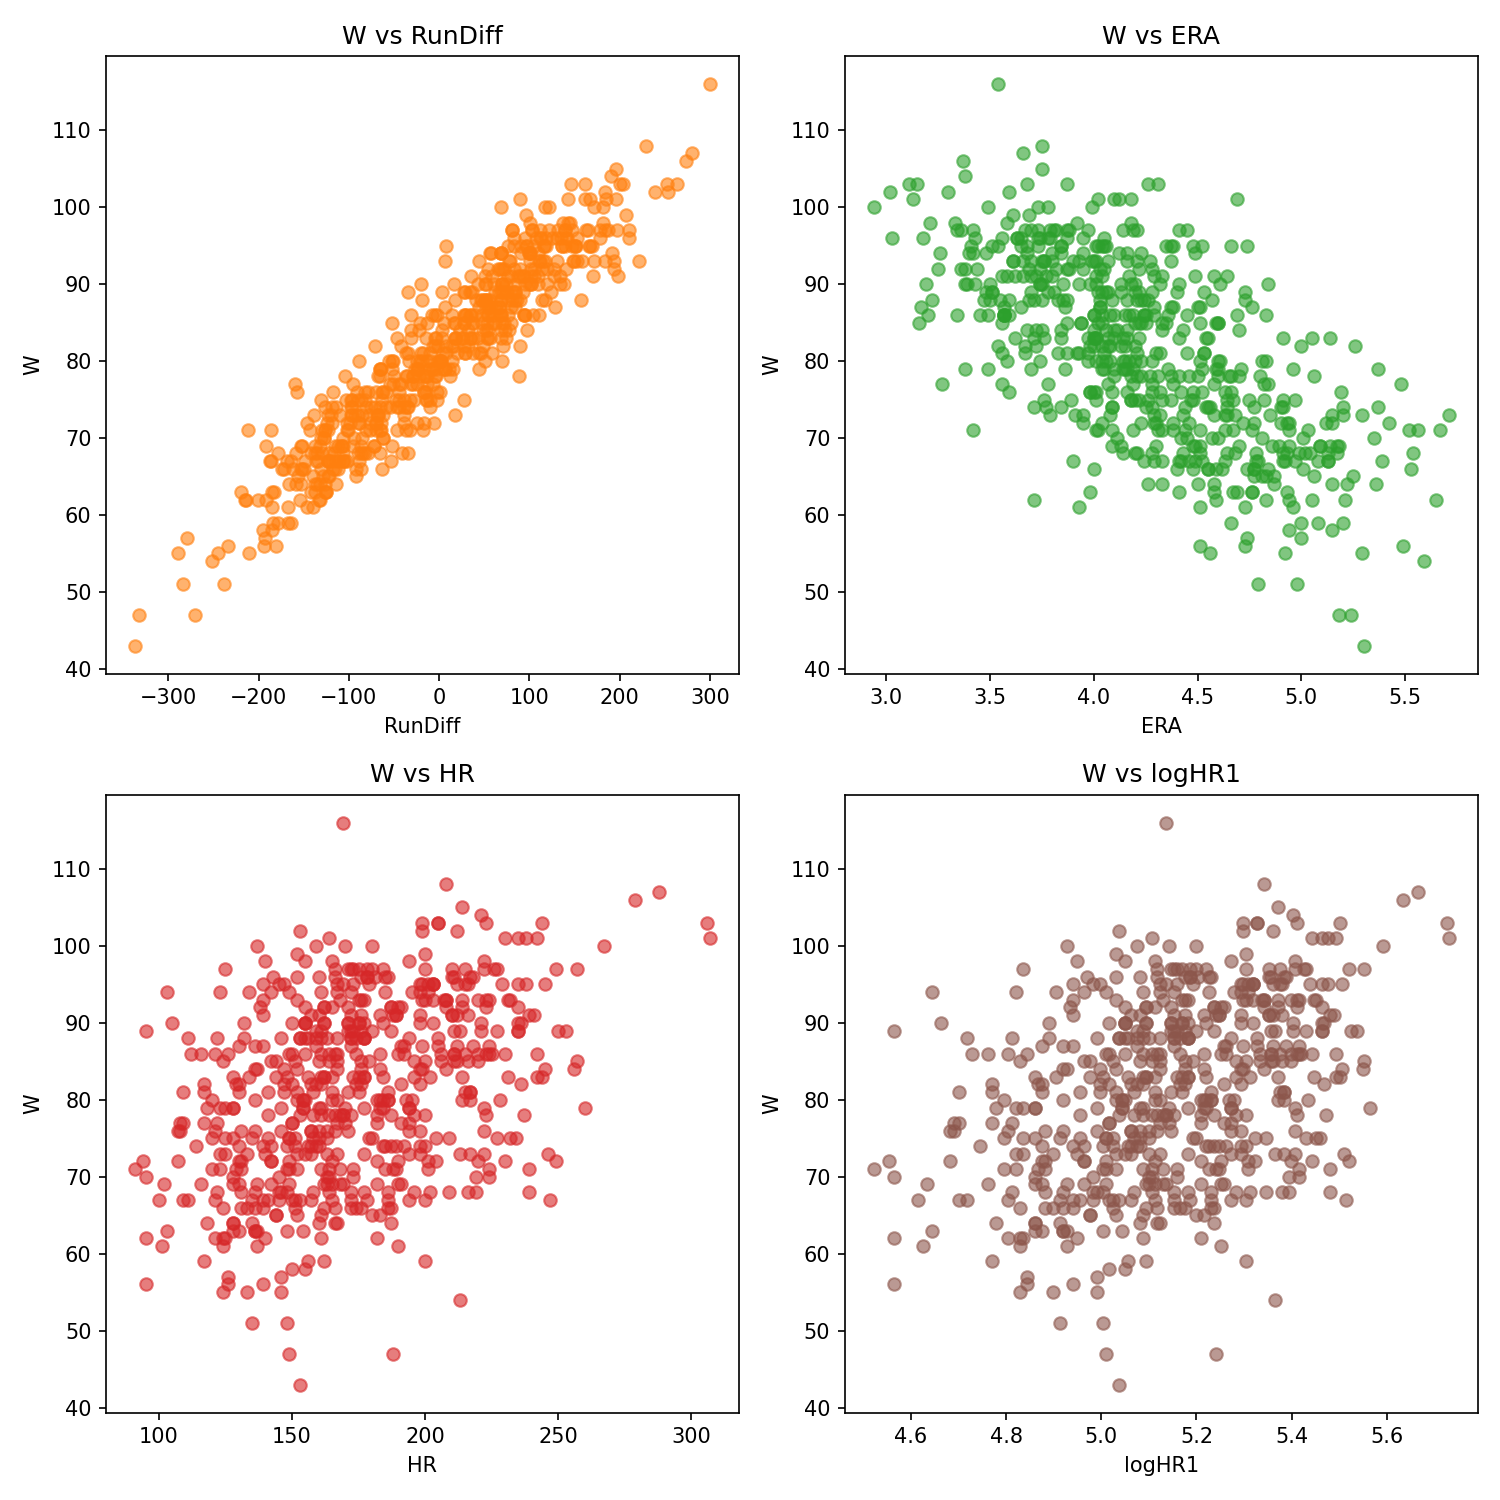
\includegraphics[width=\textwidth]{../plots/all_scatter_W.png}
    \caption{Diagramas de dispersión: W vs RunDiff, ERA, HR y log(HR+1).}
\end{figure}

\textbf{W vs RunDiff} presenta la relación más fuerte y lineal: a mayor diferencial de carreras, más victorias, confirmando su validez como predictor central.  
\textbf{W vs ERA} muestra una relación negativa clara: equipos con menor efectividad del pitcheo (ERA baja) ganan más.  
\textbf{W vs HR} y \textbf{W vs logHR1} tienen asociación positiva pero más difusa; los cuadrangulares ayudan a ganar, aunque con variabilidad, lo cual lleva a explorar transformaciones.

\begin{figure}[H]
    \centering
    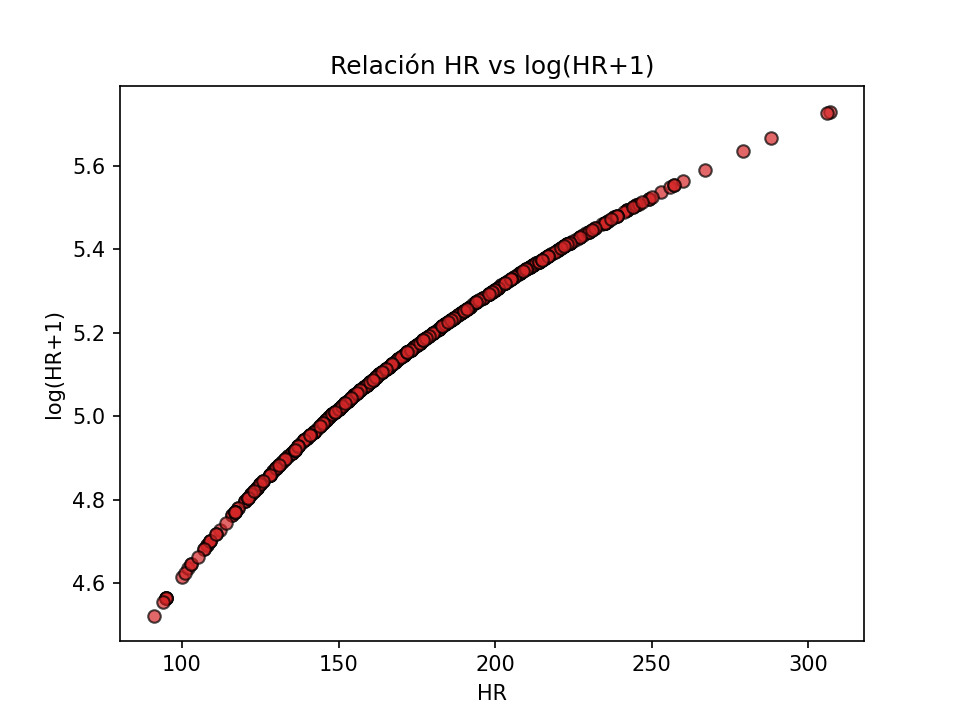
\includegraphics[width=0.75\textwidth]{../plots/scatter_HR_logHR1.png}
    \caption{Relación funcional entre HR y log(HR+1).}
\end{figure}

La curva muestra que $\log(HR+1)$ suaviza el crecimiento de los HR. 
Aunque en el rango 90-300 se mantiene casi lineal, la transformación previene que valores extremos dominen el ajuste del modelo, haciendo el análisis más robusto.

\begin{figure}[H]
    \centering
    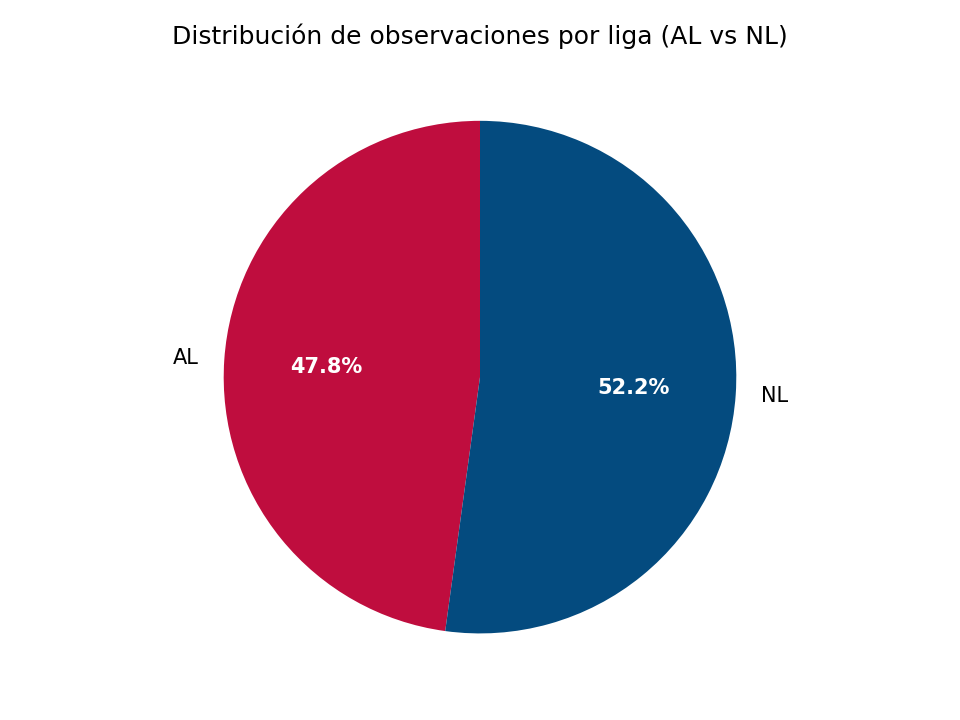
\includegraphics[width=0.6\textwidth]{../plots/pie_ligas_colored.png}
    \caption{Distribución de observaciones por liga (AL vs NL), 2000--2019.}
\end{figure}

El dataset está balanceado entre \textbf{NL} (52.2\%) y \textbf{AL} (47.8\%),y con esto se garantiza representatividad de ambas ligas, sin sesgos por desbalance en la muestra.

\begin{figure}[H]
    \centering
    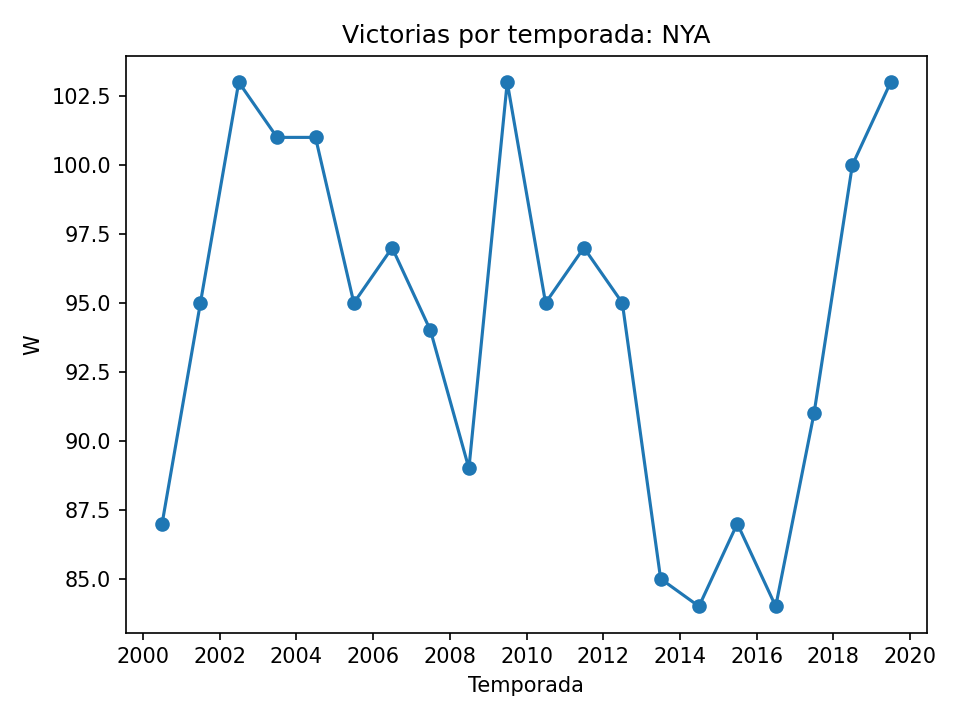
\includegraphics[width=0.8\textwidth]{../plots/ts_W_NYA.png}
    \caption{Serie de tiempo de victorias (ejemplo: NYA), 2000--2019.}
\end{figure}

Los Yankees de Nueva York (NYA) ilustran la variabilidad interanual en victorias. 
Se observan picos de más de 100 triunfos en varias temporadas y caídas a la franja de 85-90 victorias en otras. 
Este patrón muestra que incluso equipos consistentemente competitivos presentan fluctuaciones naturales, útiles para entender la estabilidad del modelo a lo largo del tiempo.

%%%%%%%%%%%%%%%%%%%%%%%%%%%%%%%%%%%%%%%%%%%%%%%%%%%%%%%%%%%%%%%%%%%%%%%%%%%%%%%%%%%%%%%%%%%%%%%%%%%%%%%%%%%%%%%%%%%%%%%%%%%%%%%%%%%%%%%%%%%%%%%%%%%%%%%%%%%%%%%%%%%%%%%%%%%%%%%%%%%%%%%%%%%%%%
\subsection{Identificación de valores atípicos:}

El análisis mediante el método del rango intercuartílico (IQR) permitió identificar observaciones atípicas en varias variables:

\begin{itemize}
    \item \textbf{Victorias (W):} El caso más extremo corresponde a los Detroit Tigers en 2003, con solo 43 victorias, claramente fuera del rango intercuartílico (45--117). Esto refleja una de las peores campañas en la historia reciente de MLB.
    \item \textbf{Jonrones (HR):} En 2019 se detectaron valores extraordinariamente altos en equipos como Minnesota Twins (307), New York Yankees (306), Houston Astros (288) y Los Angeles Dodgers (279), todos por encima del umbral superior (275.5). Esto coincide con el ``Año del jonrón''. en 2019, cuando se registró un récord colectivo histórico de cuadrangulares.
    \item \textbf{Transformación log(HR+1):} Aunque la mayoría de observaciones están dentro del rango, aparecen valores bajos en equipos con ofensivas débiles como los San Diego Padres (2011) y San Francisco Giants (2008), lo que confirma que esta transformación ayuda a suavizar pero no elimina del todo los outliers.
    \item \textbf{Carreras anotadas (R):} Se identifican equipos con valores extremos, por ejemplo, los Yankees (2007) y Rockies (2000) con más de 968 carreras, y los Marlins (2013) o Mariners (2010) con apenas 513, fuera del rango esperado (517--962).
    \item \textbf{Juegos disputados (G):} Aunque la liga establece un calendario de 162 juegos, se detectan temporadas con 161 o 163 partidos, resultado de suspensiones o reprogramaciones (e.g., Cubs 2009, Rockies 2007, Rangers 2013).
    \item \textbf{Derrotas (L):} Nuevamente destacan los Tigers de 2003, con 119 derrotas, simétrico al outlier en victorias.
\end{itemize}

Estos valores atípicos no necesariamente representan errores de medición, sino hechos históricos del béisbol (equipos en un muy bajo nivel, ofensivas históricas, o particularidades del calendario). Sin embargo, es importante tenerlos en cuenta porque pueden influir en el ajuste de los modelos de regresión, afectando los coeficientes e incrementando la dispersión residual.
%%%%%%%%%%%%%%%%%%%%%%%%%%%%%%%%%%%%%%%%%%%%%%%%%%%%%%%%%%%%%%%%%%%%%%%%%%%%%%%%%%%%%%%%%%%%%%%%%%%%%%%%%%%%%%%%%%%%%%%%%%%%%%%%%%%%%%%%%%%%%%%%%%%%%%%%%%%%%%%%%%%%%%%%%%%%%%%%%%%%%%%%%%%%%%
%%%%%%%%%%%%%%%%%%%%%%%%%%%%%%%%%%%%%%%%%%%%%%%%%%%%%%%%%%%%%%%%%%%%%%%%%%%%%%%%%%%%%%%%%%%%%%%%%%%%%%%%%%%%%%%%%%%%%%%%%%%%%%%%%%%%%%%%%%%%%%%%%%%%%%%%%%%%%%%%%%%%%%%%%%%%%%%%%%%%%%%%%%%%%%
\section{Análisis de Correlación}
\subsection{Correlación entre las variables:}

Se calculó el coeficiente de correlación de Pearson y Spearman entre el número de victorias (W) y las variables explicativas 
(RunDiff, ERA, HR y logHR1). Los resultados se resumen en la Tabla \ref{tab:corr_w_x} y en las Figuras 
\ref{fig:heatmap_pearson}--\ref{fig:heatmap_spearman}.

\begin{table}[H]
    \centering
    \caption{Correlación de W con variables explicativas}
    \label{tab:corr_w_x}
    \begin{tabular}{lrrrrr}
    \toprule
    Variable & Pearson r & p (Pearson) & Spearman $\rho$ & p (Spearman) & N \\
    \midrule
    RunDiff & 0.9395 & 0.0000 & 0.9398 & 0.0000 & 600 \\
    HR & 0.3920 & 0.0000 & 0.3853 & 0.0000 & 600 \\
    logHR1 & 0.3901 & 0.0000 & 0.3853 & 0.0000 & 600 \\
    ERA & -0.6554 & 0.0000 & -0.6575 & 0.0000 & 600 \\
    \bottomrule
    \end{tabular}
\end{table}


\begin{figure}[H]
    \centering
    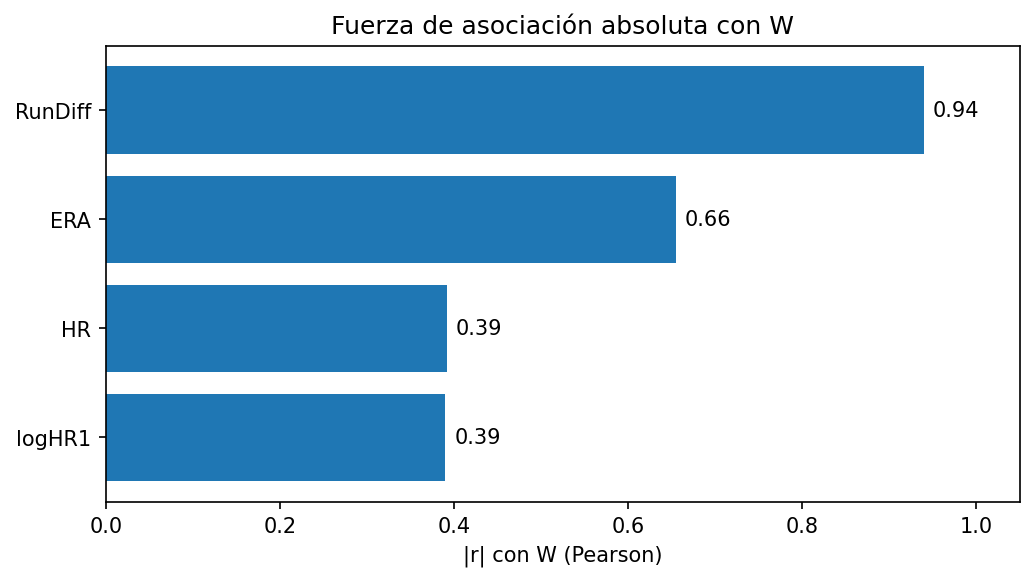
\includegraphics[width=0.75\textwidth]{../plots/bar_abs_r_W.png}
    \caption{Fuerza de asociación absoluta (|r|) de cada predictor con W (Pearson).}
    \label{fig:bar_abs_r}
\end{figure}

\begin{itemize}
    \item \textbf{RunDiff} presenta la correlación más fuerte con $W (r = 0.94, p < 0.001)$, lo que confirma que la diferencia de carreras es un predictor casi determinístico del número de victorias.
    \item \textbf{ERA} muestra una correlación negativa alta $(r = -0.66, p < 0.001)$. Esto indica que un menor promedio de carreras limpias permitidas (mejor pitcheo) está fuertemente asociado con más victorias.
    \item \textbf{HR} y su transformación \textbf{logHR1} exhiben correlaciones positivas moderadas $(r \approx 0.39, p < 0.001)$. Los jonrones ayudan a ganar partidos, aunque no explican tanto como RunDiff o ERA. La similitud entre HR y logHR1 confirma que la transformación logarítmica apenas cambia la relación en el rango observado (90--300 jonrones).
\end{itemize}

\begin{figure}[H]
    \centering
    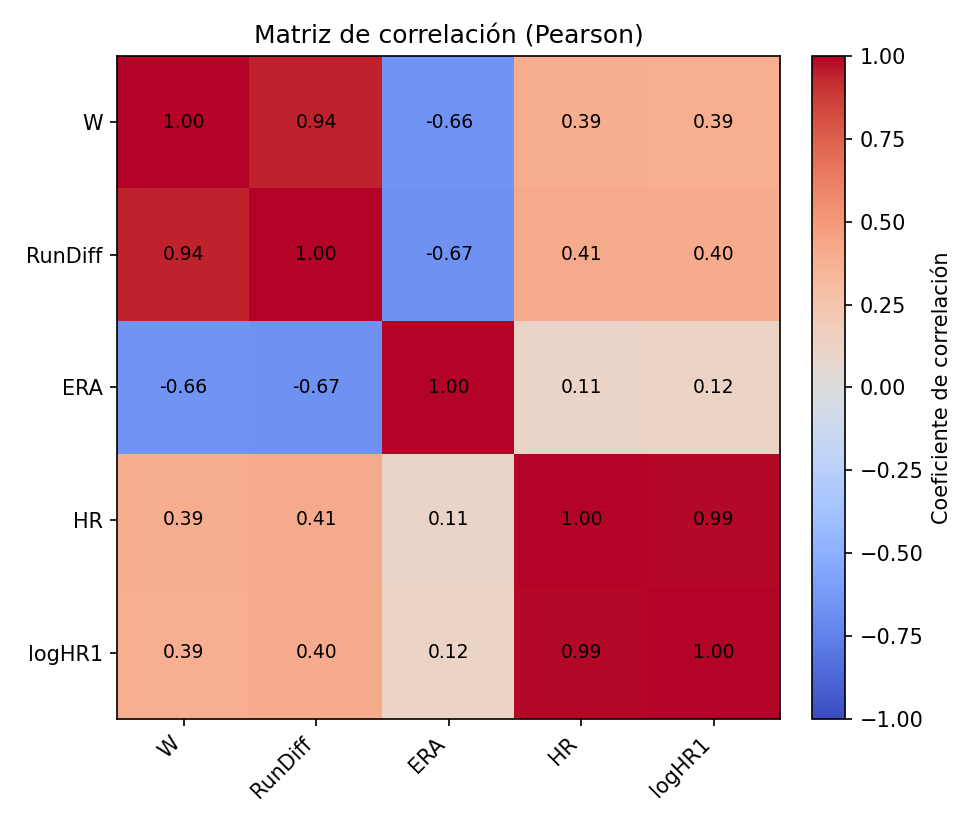
\includegraphics[width=0.6\textwidth]{../plots/heatmap_corr_pearson.png}
    \caption{Matriz de correlación (Pearson) entre W y las variables explicativas.}
    \label{fig:heatmap_pearson}
\end{figure}

\begin{figure}[H]
    \centering
    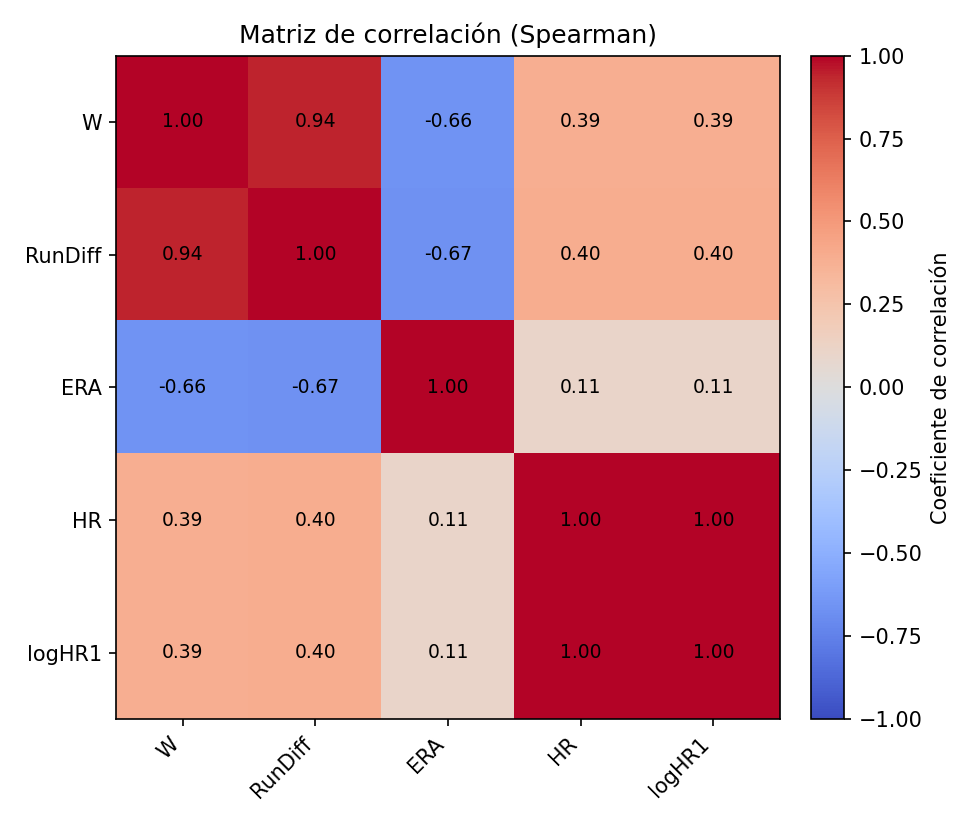
\includegraphics[width=0.6\textwidth]{../plots/heatmap_corr_spearman.png}
    \caption{Matriz de correlación (Spearman) entre W y las variables explicativas.}
    \label{fig:heatmap_spearman}
\end{figure}

Tanto Pearson como Spearman producen resultados consistentes: RunDiff y ERA son los predictores más fuertemente asociados con las victorias, mientras que los jonrones tienen un efecto más limitado. Esto anticipa que los modelos de regresión simple con RunDiff y ERA tendrán mayor poder explicativo que aquellos con HR.
%%%%%%%%%%%%%%%%%%%%%%%%%%%%%%%%%%%%%%%%%%%%%%%%%%%%%%%%%%%%%%%%%%%%%%%%%%%%%%%%%%%%%%%%%%%%%%%%%%%%%%%%%%%%%%%%%%%%%%%%%%%%%%%%%%%%%%%%%%%%%%%%%%%%%%%%%%%%%%%%%%%%%%%%%%%%%%%%%%%%%%%%%%%%%%
\section{Modelo de Regresión Simple (3 modelos)}

\subsection{Resultados y resumen de estimaciones}

Se ajustaron cuatro modelos de regresión lineal simple con \textbf{W} (victorias por temporada) 
como variable dependiente y, por separado, como variables explicativas: \textbf{RunDiff}, \textbf{ERA}, \textbf{HR} y \textbf{\(\log(\text{HR}+1)\)}. 
Los resultados completos se muestran en la Tabla~\ref{tab:ols_summary}:

\begin{table}[H]
    \caption{Modelos de regresión lineal simple: coeficientes y bondad de ajuste}
    \label{tab:ols_summary}
    \resizebox{\textwidth}{!}{
        \begin{tabular}{lrrrrrrrrrrrrrr}
            \toprule
                Modelo & $\beta_0$ & $\beta_1$ & $p(\beta_1)$ & CI95\% Inf & CI95\% Sup & $R^2$ & $R^2_{adj}$ & F & $p(F)$ & AIC & BIC & RMSE & MAE & N \\
                \midrule
                W ~ RunDiff & 80.9700 & 0.0997 & 0.0000 & 0.0967 & 0.1026 & 0.8827 & 0.8825 & 4498.4794 & 0.0000 & 3380.4384 & 3389.2322 & 4.0340 & 3.2120 & 600 \\
                W ~ ERA & 142.3221 & -14.4426 & 0.0000 & -15.7791 & -13.1060 & 0.4296 & 0.4286 & 450.3684 & 0.0000 & 4329.2274 & 4338.0212 & 8.8944 & 7.1557 & 600 \\
                W ~ HR & 59.2303 & 0.1253 & 0.0000 & 0.1017 & 0.1489 & 0.1537 & 0.1522 & 108.5754 & 0.0000 & 4565.9635 & 4574.7574 & 10.8341 & 8.9117 & 600 \\
                W ~ logHR1 & -29.3238 & 21.4615 & 0.0000 & 17.3937 & 25.5292 & 0.1522 & 0.1508 & 107.3631 & 0.0000 & 4566.9939 & 4575.7878 & 10.8434 & 8.9306 & 600 \\
            \bottomrule
        \end{tabular}
    }
\end{table}


\begin{figure}[H]
    \centering
    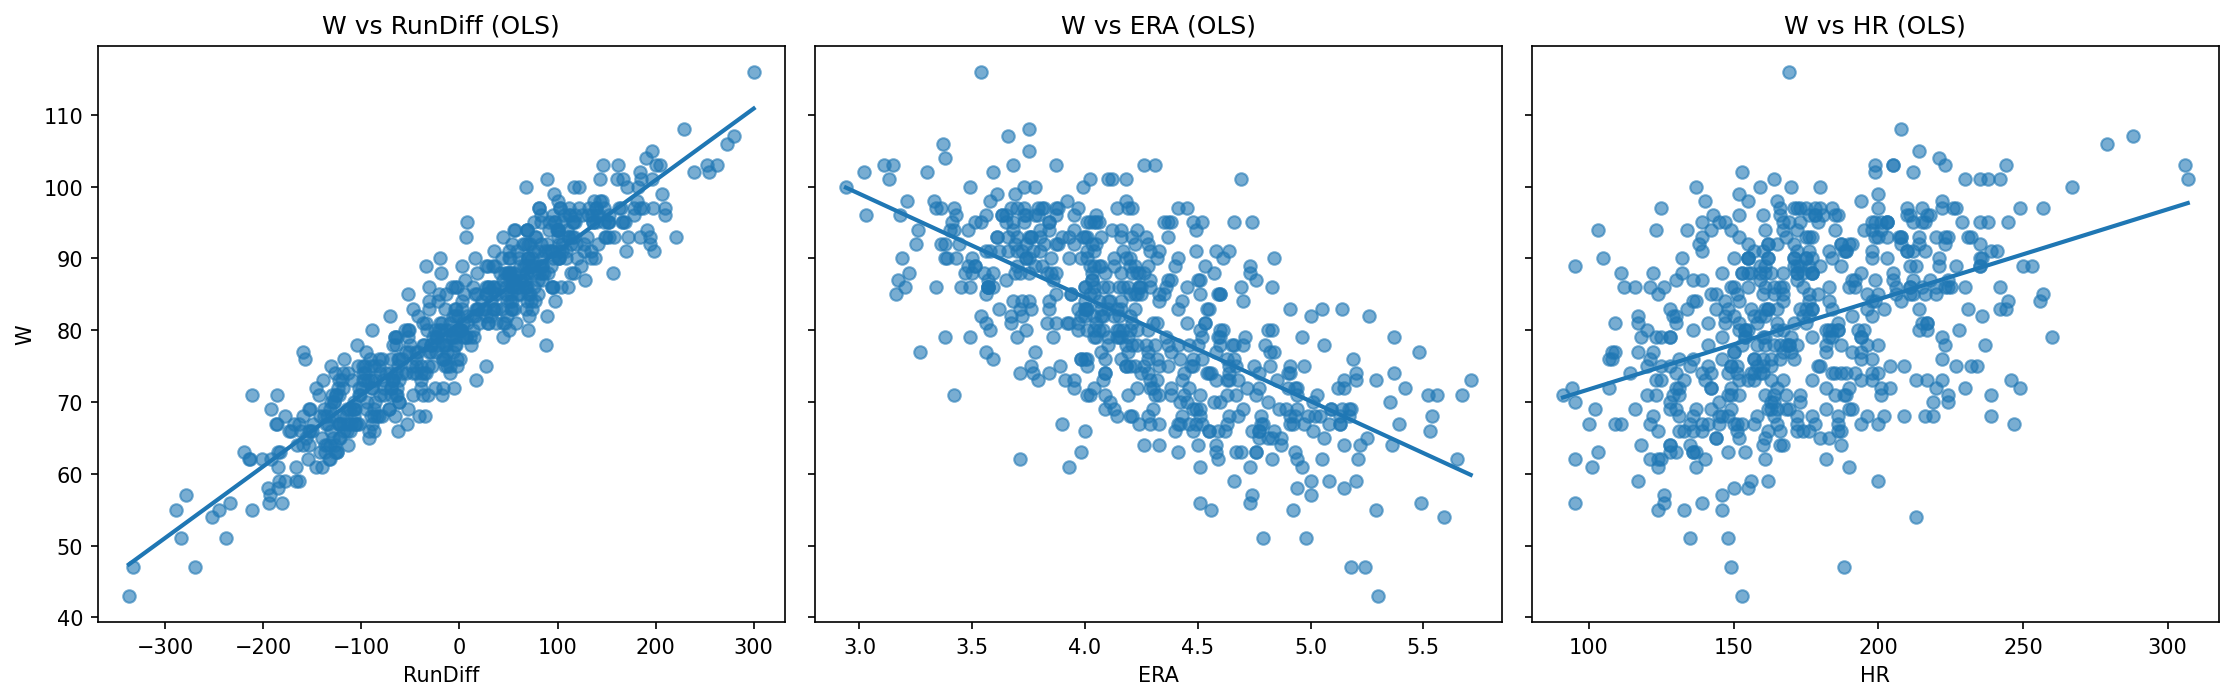
\includegraphics[width=\textwidth]{../plots/ols_scatter_grid_RunDiff_ERA_HR.png}
    \caption{Diagramas de dispersión: W vs RunDiff, ERA, HR y log(HR+1).}
\end{figure}

\begin{figure}[H]
    \centering
    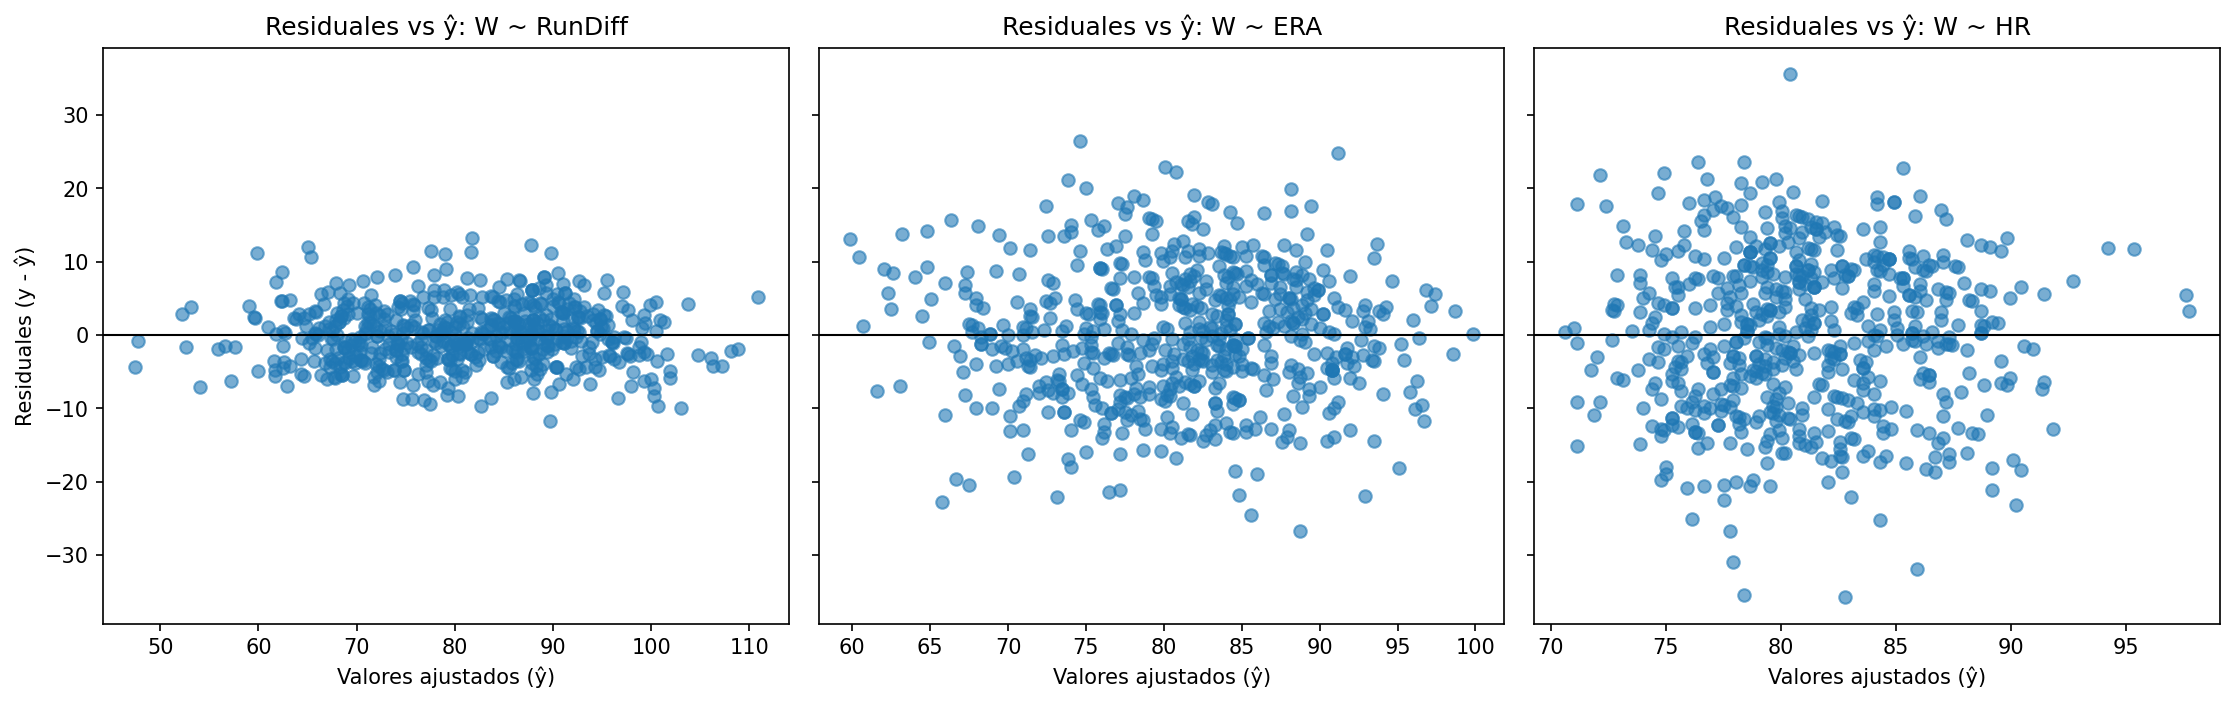
\includegraphics[width=\textwidth]{../plots/ols_resid_grid_RunDiff_ERA_HR.png}
    \caption{Residuales vs valores ajustados: W vs RunDiff, ERA, HR y log(HR+1).}
\end{figure}

\subsection{Interpretación de los resultados}

\paragraph{W \(\sim\) RunDiff.}  
Este modelo presenta un ajuste sobresaliente: \(R^2=0.883\), con un error medio de apenas 4 juegos (RMSE \(=4.03\), MAE \(=3.21\)). El coeficiente estimado de 0.0997 implica que por cada 10 carreras de diferencia anotadas sobre el rival, un equipo gana en promedio una victoria adicional. El intercepto de 80.97 refleja que un equipo “neutral” (RunDiff=0) tiende a terminar con 81 victorias, lo cual coincide con el balance teórico de .500. Este es, con diferencia, el modelo más predictivo.

\paragraph{W \(\sim\) ERA.}  
La relación entre la efectividad de los lanzadores y las victorias también es significativa (\(p<0.001\)), con una pendiente de -14.44: reducir en 1.00 la ERA equivale aproximadamente a 14 victorias adicionales. Aunque el ajuste es más modesto que con RunDiff (\(R^2=0.43\)), este modelo ofrece una visión valiosa del rol del pitcheo en el éxito global del equipo.

\paragraph{W \(\sim\) HR.}  
Cada 10 jonrones se asocian con 1.25 victorias adicionales. Sin embargo, el poder explicativo es limitado (\(R^2=0.154\), RMSE=10.83). Esto refleja que, aunque los cuadrangulares ayudan, existen múltiples caminos ofensivos para anotar que no se capturan solo con HR.

\paragraph{W \(\sim \log(\text{HR}+1)\).}  
La transformación logarítmica produce resultados prácticamente idénticos a HR lineal (\(R^2=0.152\), RMSE=10.84). Esto confirma lo observado en el análisis exploratorio: en el rango de 90–300 HR, la relación con victorias es casi lineal y la transformación no mejora el ajuste.

\subsection{Evaluación de la bondad de ajuste}

\begin{itemize}
    \item \textbf{Mejor modelo:} RunDiff domina en todos los indicadores (\(R^2\), AIC, BIC, RMSE, MAE).
    \item \textbf{Modelo intermedio:} ERA es una métrica útil, con un ajuste razonable, que complementa la interpretación sabermétrica con una perspectiva puramente de pitcheo.
    \item \textbf{Modelos débiles:} HR y \(\log(HR+1)\) muestran asociaciones significativas pero débiles, explicando solo un 15\% de la variabilidad de W.
    \item \textbf{Pruebas de significancia:} En todos los casos, la prueba F global confirma que los modelos son estadísticamente significativos (\(p<0.001\)).
    \item \textbf{Error de predicción:} Con RunDiff, el error típico es de $\approx 3\text{--}4$ victorias por temporada; con ERA, sube a $\approx 7\text{--}9$; con HR, a casi $\approx 9\text{--}11$.
\end{itemize}

\noindent Bajo este análisis, se puede concluir que el diferencial de carreras es el mejor predictor de victorias. Sin embargo, ERA aporta información clave sobre la importancia del pitcheo, mientras que los jonrones reflejan solo una parte limitada de la ofensiva.
%%%%%%%%%%%%%%%%%%%%%%%%%%%%%%%%%%%%%%%%%%%%%%%%%%%%%%%%%%%%%%%%%%%%%%%%%%%%%%%%%%%%%%%%%%%%%%%%%%%%%%%%%%%%%%%%%%%%%%%%%%%%%%%%%%%%%%%%%%%%%%%%%%%%%%%%%%%%%%%%%%%%%%%%%%%%%%%%%%%%%%%%%%%%%%
\section{Formas Funcionales}
Para cada predictor probamos una forma lineal y una alternativa no lineal:\\
\begin{enumerate}
    \item \textbf{HR} vs.\ \(\log(\text{HR}+1)\); 
    \item \textbf{ERA} lineal vs.\ cuadrática \((\text{ERA}^2)\); 
    \item \textbf{RunDiff} lineal vs.\ cuadrática \((\text{RunDiff}^2)\).
\end{enumerate}
La comparación se basó en \(R^2\), \(R^2_{adj}\), AIC/BIC, RMSE in--sample y RMSE de validación cruzada (10-fold), además de diagnósticos Breusch--Pagan (heterocedasticidad) y RESET de Ramsey (no linealidades u omisiones).

\begin{table}[H]
    \caption{Comparación de formas funcionales por predictor}
    \label{tab:formas_funcionales}
    \resizebox{\textwidth}{!}{
        \begin{tabular}{lrrrrrrrrrrrrrr}
            \toprule
                Modelo & $k$ & $R^2$ & $R^2_{adj}$ & AIC & BIC & RMSE & MAE & RMSE$_{CV}$ (media) & RMSE$_{CV}$ (sd) & BP F & $p$(BP) & RESET F & $p$(RESET) & N \\
            \midrule
                W ~ HR & 1 & 0.1537 & 0.1522 & 4565.9635 & 4574.7574 & 10.8341 & 8.9117 & 10.8372 & 0.6868 & 0.6344 & 0.4261 & 0.3085 & 0.7346 & 600 \\
                W ~ log(HR+1) & 1 & 0.1522 & 0.1508 & 4566.9939 & 4575.7878 & 10.8434 & 8.9306 & 10.8479 & 0.6725 & 0.3728 & 0.5417 & 0.5937 & 0.5526 & 600 \\
                W ~ ERA & 1 & 0.4296 & 0.4286 & 4329.2274 & 4338.0212 & 8.8944 & 7.1557 & 8.8994 & 0.4535 & 2.6423 & 0.1046 & 4.1149 & 0.0168 & 600 \\
                $W \sim ERA + ERA^2$ & 2 & 0.4296 & 0.4277 & 4331.2180 & 4344.4088 & 8.8943 & 7.1572 & 8.9189 & 0.4407 & 2.4197 & 0.0898 & 5.4130 & 0.0047 & 600 \\
                W ~ RunDiff & 1 & 0.8827 & 0.8825 & 3380.4384 & 3389.2322 & 4.0340 & 3.2120 & 4.0259 & 0.4107 & 0.0072 & 0.9322 & 3.5185 & 0.0303 & 600 \\
                $W \sim \text{RunDiff} + \text{RunDiff}^2$ & 2 & 0.8835 & 0.8831 & 3378.1195 & 3391.3103 & 4.0195 & 3.1946 & 4.0256 & 0.3990 & 0.0806 & 0.9226 & 1.6484 & 0.1932 & 600 \\
            \bottomrule
        \end{tabular}
    }
\end{table}


\begin{figure}[H]\centering
    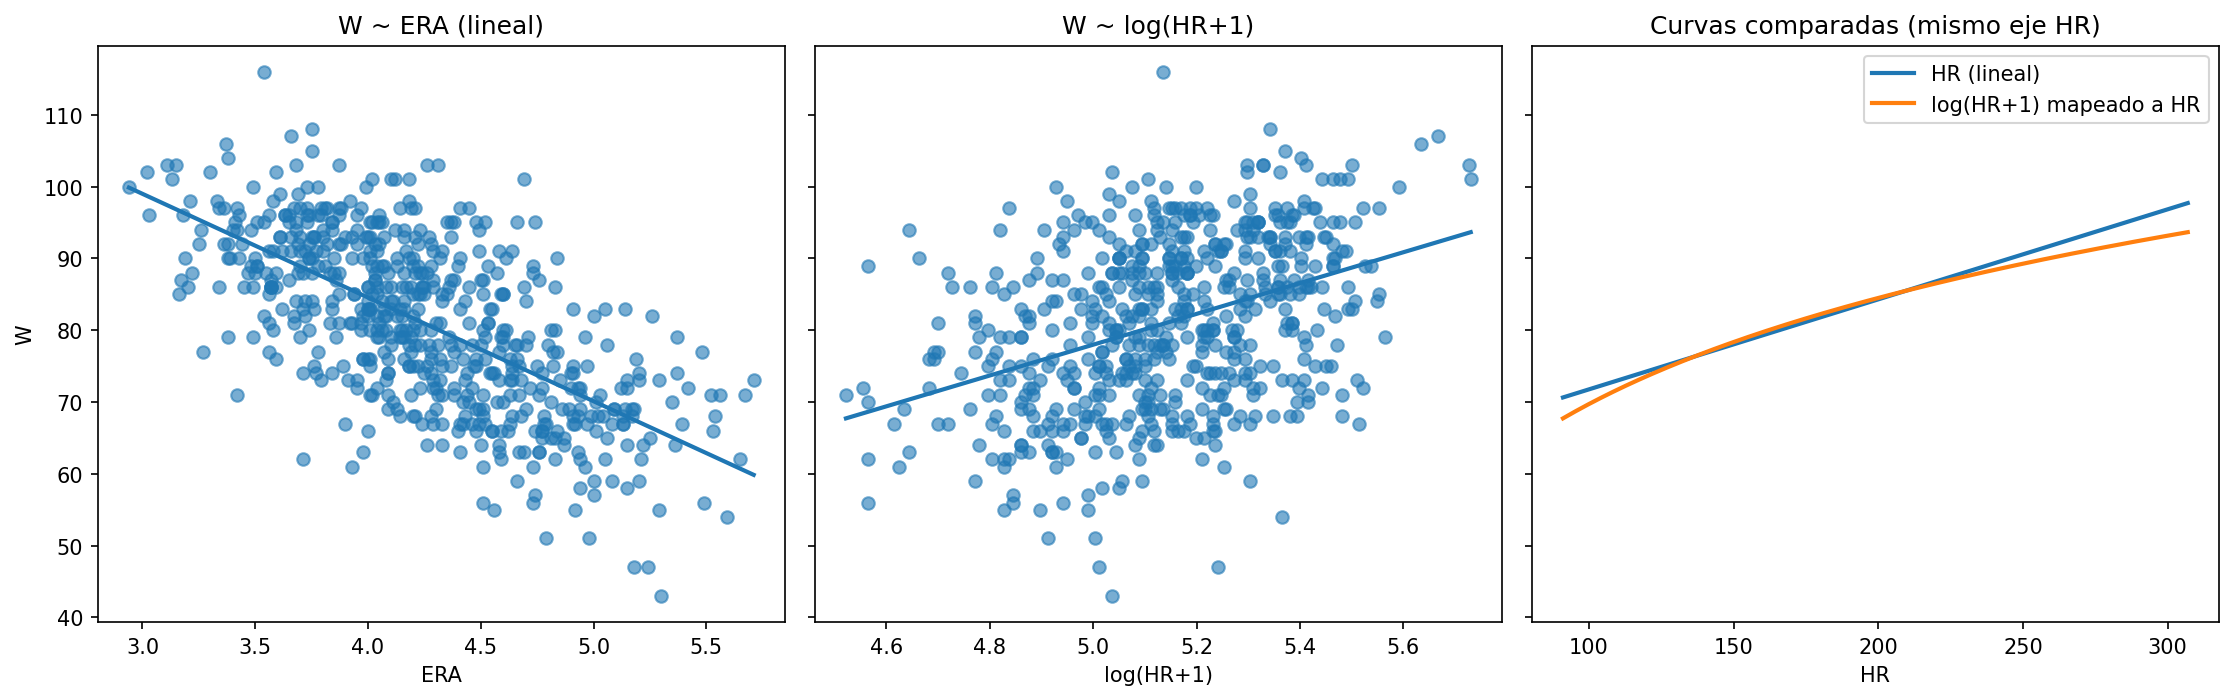
\includegraphics[width=\textwidth]{../plots/formas_funcionales_HR.png}
    \caption{HR: comparación lineal vs.\ \(\log(\text{HR}+1)\).}
    \label{fig:ff_hr}
\end{figure}

\begin{figure}[H]\centering
    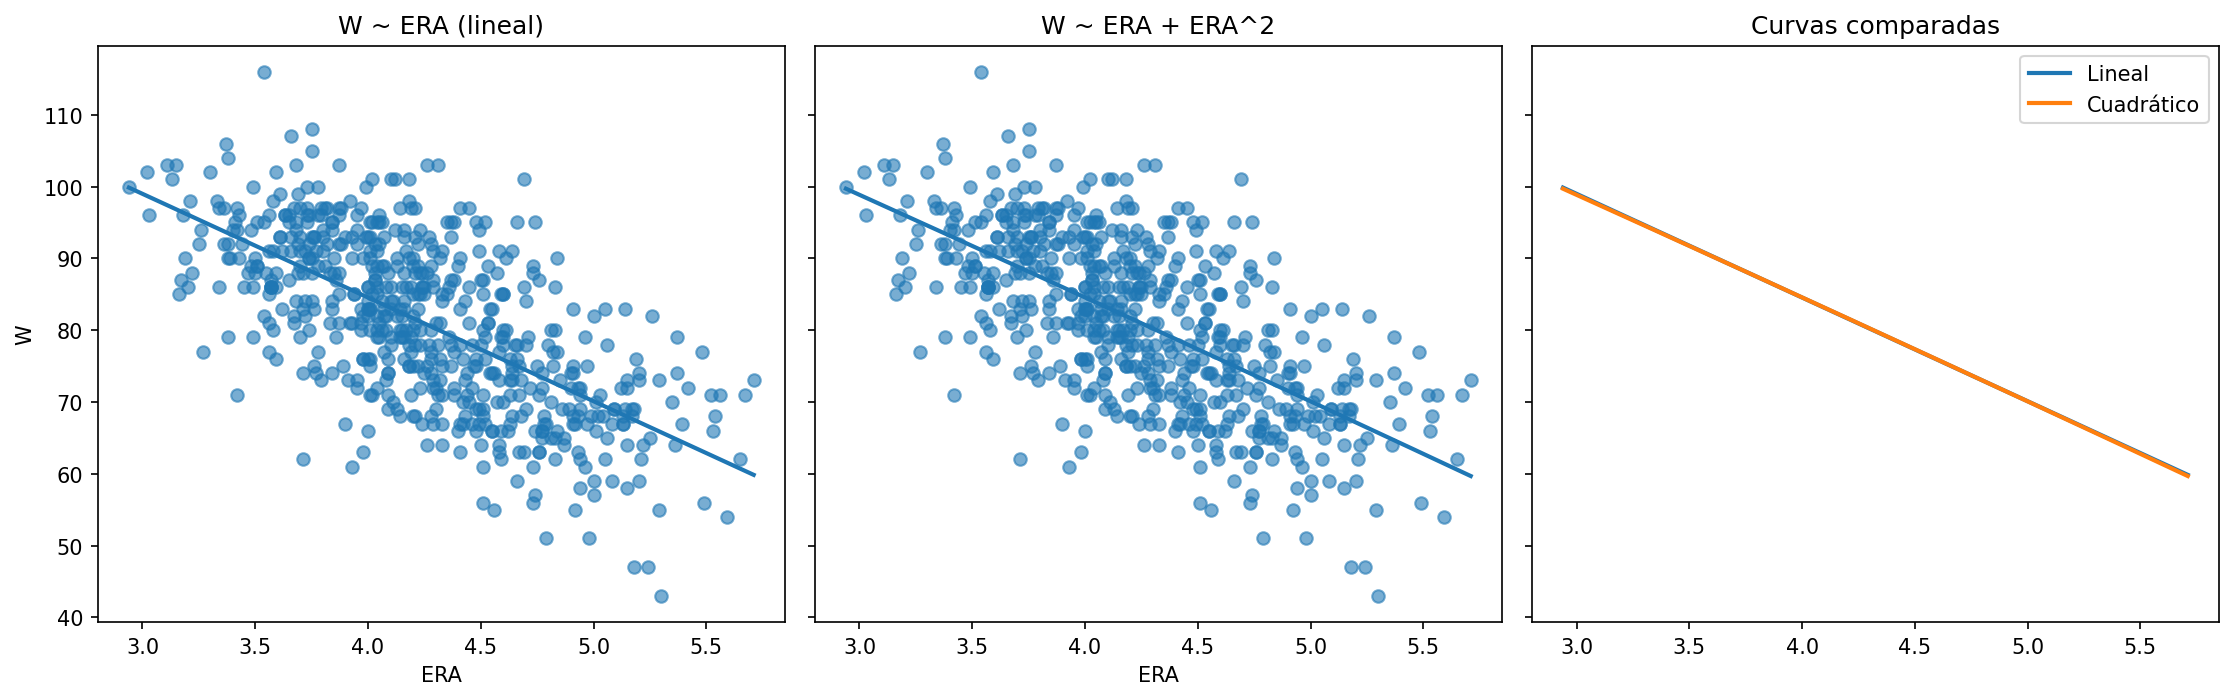
\includegraphics[width=\textwidth]{../plots/formas_funcionales_ERA.png}
    \caption{ERA: comparación lineal vs.\ cuadrática.}
    \label{fig:ff_era}
\end{figure}
    
    \begin{figure}[H]\centering
    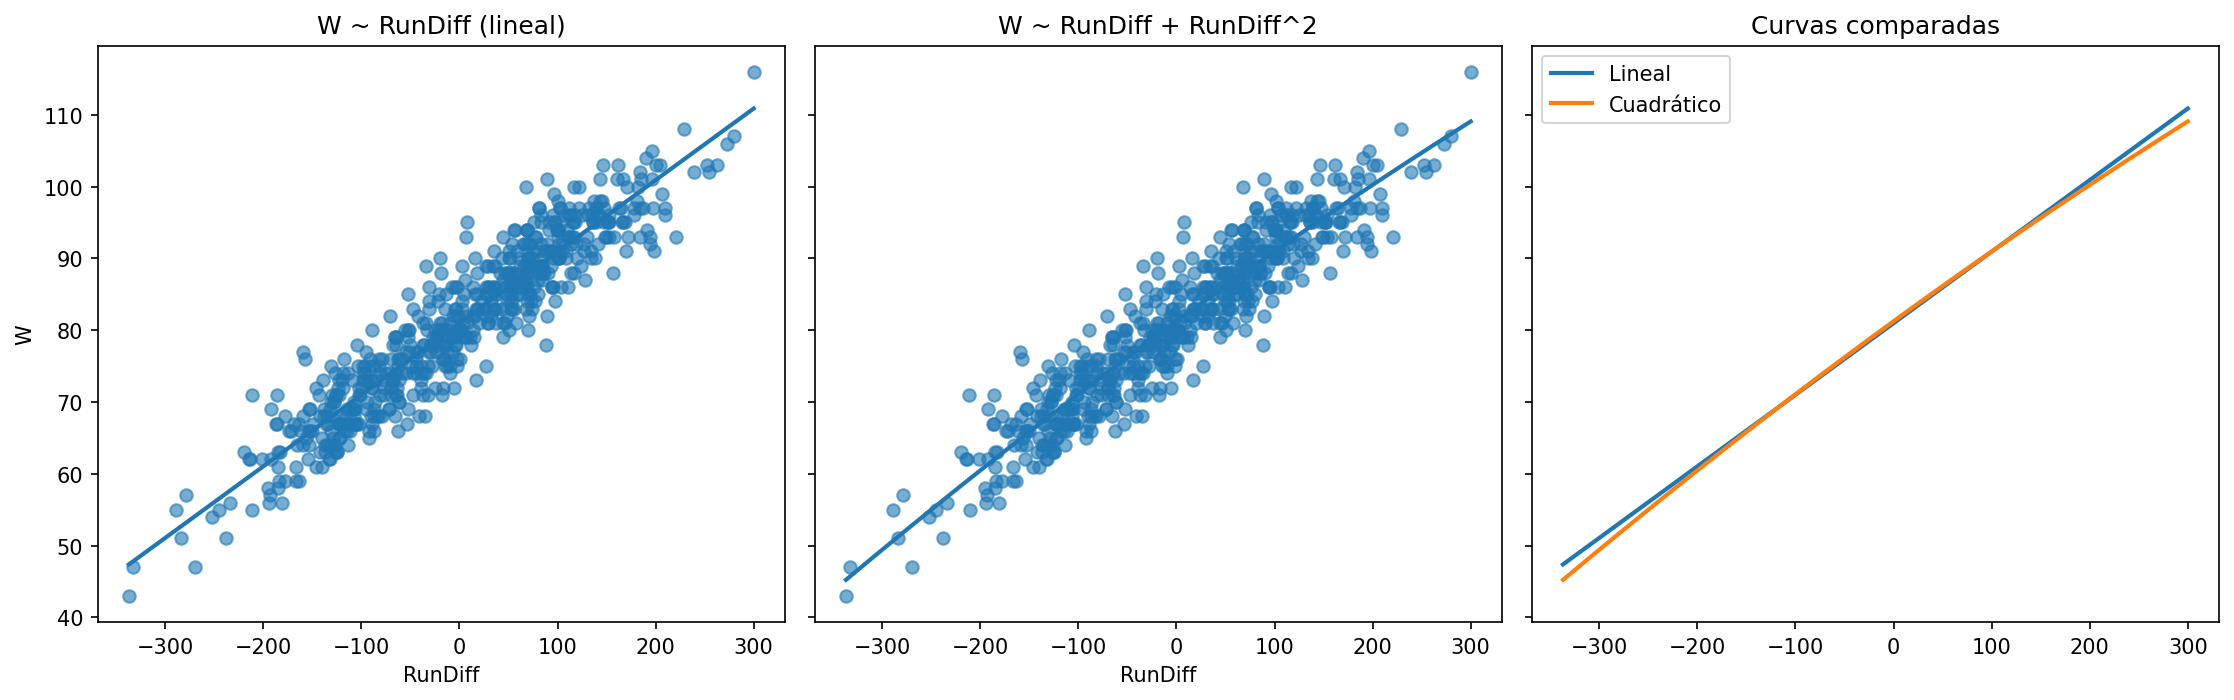
\includegraphics[width=\textwidth]{../plots/formas_funcionales_RunDiff.png}
    \caption{RunDiff: comparación lineal vs.\ cuadrática.}
    \label{fig:ff_rundiff}
\end{figure}

\subsection{Resultados e interpretación}

    \paragraph{HR (\(W \sim HR\) vs.\ \(W \sim \log(\text{HR}+1)\)).}
    Las métricas son prácticamente idénticas entre la forma lineal y la logarítmica: \(R^2 \approx 0.153\), RMSE \(\approx 10.84\) y AIC/BIC casi iguales. 
    Ni el test RESET (p=0.59 para log y p=0.31 para lineal) ni Breusch--Pagan (p\(\approx 0.37{-}0.54\)) sugieren problemas de especificación u heterocedasticidad. 
    \textit{Conclusión:} la transformación \(\log(\text{HR}+1)\) \textbf{no aporta mejora} sustantiva; mantenemos \textbf{HR lineal} como especificación base y usamos la versión logarítmica sólo como contraste funcional.

    \paragraph{ERA (\(W \sim \text{ERA}\) vs.\ \(W \sim \text{ERA}+\text{ERA}^2\)).}
    El término cuadrático no mejora el ajuste: \(R^2\) se mantiene (0.4296 vs.\ 0.4296), AIC/BIC \textit{empeoran} levemente con el cuadrático, y el RMSE-CV también es ligeramente mayor (8.92 vs.\ 8.90). 
    RESET es significativo en ambas (p=0.0168 lineal; p=0.0047 cuadrática), por lo que la curvatura de segundo grado \textbf{no} corrige del todo la posible omisión de forma o variables. 
    BP no detecta heterocedasticidad (p\(\approx 0.09{-}0.10\)). 
    \textit{Conclusión:} \textbf{era suficiente la forma lineal} para ERA; incorporar \(\text{ERA}^2\) no justifica la mayor complejidad.

    \paragraph{RunDiff (\(W \sim \text{RunDiff}\) vs.\ \(W \sim \text{RunDiff}+\text{RunDiff}^2\)).}
    Aquí sí aparece una \textit{mejora pequeña pero consistente}: el \(R^2\) sube de 0.8827 a 0.8835, AIC baja (3380.44 \(\rightarrow\) 3378.12), RMSE disminuye (4.034 \(\rightarrow\) 4.020) y el RESET deja de ser significativo (p=0.0303 \(\rightarrow\) 0.193), lo que sugiere que el término cuadrático captura una leve curvatura. BP no señala heterocedasticidad. 
    \textit{Conclusión:} \textbf{RunDiff cuadrático} ofrece el mejor compromiso (ligera mejora de ajuste y especificación más estable), aunque el \textit{gain} es modesto.

\subsection{Validación del modelo transformado}

    Con base en los resultados anteriores y en las Figuras~\ref{fig:ff_hr}--\ref{fig:ff_rundiff}, seleccionamos como especificaciones finales por predictor:
    \begin{itemize}
        \item \(W \sim \text{RunDiff} + \text{RunDiff}^2\) (mejor AIC y RESET no significativo).
        \item \(W \sim \text{ERA}\) (lineal; el término cuadrático no mejora).
        \item \(W \sim \text{HR}\) (lineal; la versión logarítmica es equivalente en ajuste).
    \end{itemize}
%%%%%%%%%%%%%%%%%%%%%%%%%%%%%%%%%%%%%%%%%%%%%%%%%%%%%%%%%%%%%%%%%%%%%%%%%%%%%%%%%%%%%%%%%%%%%%%%%%%%%%%%%%%%%%%%%%%%%%%%%%%%%%%%%%%%%%%%%%%%%%%%%%%%%%%%%%%%%%%%%%%%%%%%%%%%%%%%%%%%%%%%%%%%%%
\section{Evaluación del Modelo de Regresión}
\subsection{Pruebas de significancia:}
Realizar las pruebas estadísticas necesarias para evaluar la significancia global del modelo (prueba \(F\)) y la significancia de cada coeficiente individual (pruebas \(t\)).
%%%%%%%%%%%%%%%%%%%%%%%%%%%%%%%%%%%%%%%%%%%%%%%%%%%%%%%%%%%%%%%%%%%%%%%%%%%%%%%%%%%%%%%%%%%%%%%%%%%%%%%%%%%%%%%%%%%%%%%%%%%%%%%%%%%%%%%%%%%%%%%%%%%%%%%%%%%%%%%%%%%%%%%%%%%%%%%%%%%%%%%%%%%%%%
%% TODO
\section{Pronóstico}
\subsection{Generación del pronóstico:}
Usar el modelo ajustado para realizar predicciones de la variable dependiente.

\subsection{Intervalos de predicción:}
Obtener intervalos de confianza o predicción para las futuras observaciones de la variable dependiente.

\subsection{Evaluación del pronóstico:}
Comparar las predicciones con los valores reales (si están disponibles) utilizando medidas de error como el MSE (Error Cuadrático Medio), RMSE (Raíz del MSE), y el MAE (Error Absoluto Medio).
%%%%%%%%%%%%%%%%%%%%%%%%%%%%%%%%%%%%%%%%%%%%%%%%%%%%%%%%%%%%%%%%%%%%%%%%%%%%%%%%%%%%%%%%%%%%%%%%%%%%%%%%%%%%%%%%%%%%%%%%%%%%%%%%%%%%%%%%%%%%%%%%%%%%%%%%%%%%%%%%%%%%%%%%%%%%%%%%%%%%%%%%%%%%%%
%% TODO
\section{Conclusiones}
\subsection{Resumen de los hallazgos:}
Resumir los resultados obtenidos del análisis de regresión, incluyendo la relación entre las variables y la efectividad del modelo.

\subsection{Recomendaciones:}
Si es aplicable, proporcionar recomendaciones basadas en los resultados del análisis de regresión.
%%%%%%%%%%%%%%%%%%%%%%%%%%%%%%%%%%%%%%%%%%%%%%%%%%%%%%%%%%%%%%%%%%%%%%%%%%%%%%%%%%%%%%%%%%%%%%%%%%%%%%%%%%%%%%%%%%%%%%%%%%%%%%%%%%%%%%%%%%%%%%%%%%%%%%%%%%%%%%%%%%%%%%%%%%%%%%%%%%%%%%%%%%%%%%
\section{Bibliografía}
Lahman Baseball Database -Society for American Baseball Research. (2025). Sabr.org. \url{https://sabr.org/lahman-database/}
%%%%%%%%%%%%%%%%%%%%%%%%%%%%%%%%%%%%%%%%%%%%%%%%%%%%%%%%%%%%%%%%%%%%%%%%%%%%%%%%%%%%%%%%%%%%%%%%%%%%%%%%%%%%%%%%%%%%%%%%%%%%%%%%%%%%%%%%%%%%%%%%%%%%%%%%%%%%%%%%%%%%%%%%%%%%%%%%%%%%%%%%%%%%%%
%%%%%%%%%%%%%%%%%%%%%%%%%%%%%%%%%%%%%%%%%%%%%%%%%%%%%%%%%%%%%%%%%%%%%%%%%%%%%%%%%%%%%%%%%%%%%%%%%%%%%%%%%%%%%%%%%%%%%%%%%%%%%%%%%%%%%%%%%%%%%%%%%%%%%%%%%%%%%%%%%%%%%%%%%%%%%%%%%%%%%%%%%%%%%%
\section{Anexo}
\subsection{Link al repositorio con código fuente y salidas correspondientes}
\url{https://github.com/enriquegomeztagle/MCD-ProyectoFinalEconometria-DeterminantesVictoriasMLB}
%%%%%%%%%%%%%%%%%%%%%%%%%%%%%%%%%%%%%%%%%%%%%%%%%%%%%%%%%%%%%%%%%%%%%%%%%%%%%%%%%%%%%%%%%%%%%%%%%%%%%%%%%%%%%%%%%%%%%%%%%%%%%%%%%%%%%%%%%%%%%%%%%%%%%%%%%%%%%%%%%%%%%%%%%%%%%%%%%%%%%%%%%%%%%%
%%%%%%%%%%%%%%%%%%%%%%%%%%%%%%%%%%%%%%%%%%%%%%%%%%%%%%%%%%%%%%%%%%%%%%%%%%%%%%%%%%%%%%%%%%%%%%%%%%%%%%%%%%%%%%%%%%%%%%%%%%%%%%%%%%%%%%%%%%%%%%%%%%%%%%%%%%%%%%%%%%%%%%%%%%%%%%%%%%%%%%%%%%%%%%
\end{document}
%%%%%%%%%%%%%%%%%%%%%%%%%%%%%%%%%%%%%%%%%%%%%%%%%%%%%%%%%%%%%%%%%%%%%%%%%%%%%%%%%%%%%%%%%%%%%%%%%%%%%%%%%%%%%%%%%%%%%%%%%%%%%%%%%%%%%%%%%%%%%%%%%%%%%%%%%%%%%%%%%%%%%%%%%%%%%%%%%%%%%%%%%%%%%%
